\documentclass{TP}
\usepackage[american]{babel}
\usepackage[utf8]{inputenc}
\usepackage[T1]{fontenc}
\usepackage{graphicx}
\usepackage{amsmath}
\usepackage[all]{xy}
\usepackage{hyperref}
\usepackage{todonotes}
\usepackage{placeins}
\usepackage{algorithm}
\usepackage{algpseudocode}

\graphicspath{{images/} {figs/}}

\newcommand*{\matminus}{%
  \leavevmode
  \hphantom{0}%
  \llap{%
    \settowidth{\dimen0 }{$0$}%
    \resizebox{1.1\dimen0 }{\height}{$-$}%
  }%
}

\usepackage{listings}

\lstdefinestyle{customC}{
  belowcaptionskip=1\baselineskip,
  breaklines=true,
  xleftmargin=\parindent,
  language=C,
  showstringspaces=false,
  basicstyle=\tiny\ttfamily,
  keywordstyle=\bfseries\color[rgb]{0.580, 0.000, 0.827},
  %{purple!40!lightgray},
  commentstyle=\itshape\color{green!40!black},
  identifierstyle=\bfseries\color{cyan!75!black},
  stringstyle=\color{orange},
  deletekeywords={double,float},
  classoffset=1, % starting new class
  otherkeywords={double,float},
  morekeywords={double,float},
  keywordstyle=\bfseries\color{green!55!black},
  classoffset=0
}


\usepackage[parfill]{parskip}

\title{
\includegraphics[keepaspectratio, scale=0.4]{verificarlo-logo.pdf}\\[4mm]
  Tutorial}

\hypersetup{pdftitle={Verificarlo Tutorial}}

\author{eric.petit@intel.com; pablo.oliveira@uvsq.fr; yohan.chatelain@uvsq.fr;
  francois.fevotte@edf.fr; bruno.lathuiliere@edf.fr}

\date{Université de Versailles Saint-Quentin en Yvelines - Intel - EDF}

\begin{document}
\maketitle

\centerline{\url{https://github.com/verificarlo/verificarlo}}
\tableofcontents


\section{Verificarlo Basics}

To debug or optimize floating-point computation with Verificarlo, the first
step is to compile your program with it. Verificarlo is built as a set of LLVM
plugins; to compile a program with verificarlo you should use the \texttt{verificarlo}
command instead of the usual \texttt{clang}, \texttt{icc} or \texttt{gcc}.

Once a program is compiled with Verificarlo, you can load various backends to
simulate round-off noise or the effect of lower floating-point precisions.  To
select and configure the backends that will be used, one defines the
\texttt{VFC\_BACKENDS} environment variable.

This tutorial will guide you on how to use Verificarlo, when in doubt the
documentation is available at \url{https://github.com/verificarlo/verificarlo}.

In this tutorial, we will use the docker container available at
\url{https://hub.docker.com/r/verificarlo/verificarlo/}.
To pull the latest container with verificarlo and start working with it on
the tutorial workspace type the following commands,
\begin{verbatim}
$ wget <address of verificarlo-tutorial.tar.gz>
$ tar xzvf verificarlo-tutorial.tar.gz
$ cd verificarlo-tutorial/
$ docker pull verificarlo/verificarlo
$ docker run -v $PWD:/workdir -it verificarlo/verificarlo bash
\end{verbatim}

\begin{question}
  Start the docker container and ensure you can run the \texttt{verificarlo} command,
\begin{verbatim}
$ verificarlo --help
\end{verbatim}
\end{question}

%% Uncomment below lines to include the Polynomial analysis
\section{Practical exercise: About polynomial evaluation}

Polynomial evaluation is a common source of computational error. In particular, they are used for function interpolation in libraries or user codes. As we will see, the various representation of the same polynomial do not have the same behavior in terms of performance, but also in term of numerical accuracy!

This tutorial is using the following Tchebychev polynomial from ~\cite[pp.52-54]{parker1997monte}:

$$T(x)=\sum_{i=0}^{10}{a_i \times x^{2i}}$$
With:
$a_i \in [
  1,
  \matminus 200,
  6600,
  \matminus 84480,
  549120,
  \matminus 2050048,
  4659200,
  \matminus 6553600,
  5570560,
  \matminus 2621440,
  524288
]$

We are interested in evaluating  $T$ near $1$.
This example is discussed with details in~\cite[pp.52-54]{parker1997monte}.

\subsection{Expanded form evaluation}

\subsubsection{Your first step with Verificarlo}

In this first approach, we will evaluate the polynomial in its expanded (monomial) form as given in the previous section. % Why monomial?
We first evaluate it in single precision.

\begin{question}
  \begin{enumerate}[(a)]
  \item Open the {\tt tchebychev.c} file and observe the function {\tt REAL expanded(REAL x)}.

  \item Compile {\tt tchebychev.c} with {\tt verificarlo} using the following command:

    {\tt verificarlo -{}-verbose -D FLOAT tchebychev.c -o tchebychev}

  \item Update the environment variable to use the {\tt QUAD} backend with {\tt MCA} mode and virtual precision of {\tt 24}.
  \item Execute the program multiple time with  $x=0.99$ using the command : \newline
{\tt ./tchebychev 0.99 EXPANDED} \newline
What can you observe?
  \end{enumerate}
\end{question}



\begin{question}
  \begin{enumerate}[(a)]
  \item Recompile with verificarlo the program in double precision using the command

    {\tt verificarlo -D DOUBLE tchebychev.c -o tchebychev} \\
   Check that the environment variable are still in the same configuration than in question 1.
  \item Execute the program multiple time in $x=0.99$ using the command : {\tt ./tchebychev 0.99 EXPANDED}. \newline
What can you observe?
  \end{enumerate}
\end{question}

No recompilation is required to change the analysis mode and another virtual precision.

\begin{question}
  \begin{enumerate}[(a)]
  \item Update the environment variable to use the {\tt QUAD} backend with  {\tt MCA} mode and virtual precision  {\tt 53}.
  \item Execute the program again in $x=0.99$ using the command : {\tt ./tchebychev 0.99 EXPANDED}. \newline
What can you observe?
  \end{enumerate}
\end{question}

\subsubsection{First numerical quality analysis of the polynomial evaluation}

In this section, we propose you to analyze the numerical quality of the results computed by the expanded evaluation of the polynomial. To simplify this task, a large part of the verificarlo command to execute is automated in the script~\texttt{run.sh}. The visualization is done using~\texttt{plot.py} script.






\begin{question}
  \begin{enumerate}[(a)]
 \item Open {\tt run.sh} and analyze how it works. We will emulate the single precision using the virtual precision of verificarlo.
  \item Modify {\tt run.sh} to evaluate the polynomial in the interval $[0.5,1]$ by $0.001$ step.
  \item Open {\tt plot.py} and analyze how it works, in particular the data that will be plotted.
  \end{enumerate}
\end{question}









The \texttt{plot.py} script generates plot similar to
figure~\ref{fig:expanded:double:24}.
The upper part of the figure represents the number $s$ of significant digits of the results: $s=-\log_{10}\left|\dfrac{\hat\sigma}{\hat\mu}\right|$ with $\hat\sigma$ the sample empirical standard deviation  $\hat\mu$ their average.


The central part is the empirical standard deviation $\hat\sigma$ for each value of $x$.

Finally the lowest parts are the $T(x)$ samples and their average in dotted line. The 20 Monte Carlo samples $T(x)$ are plotted for each $x$ value (sometime overlapping on the graphic)

\begin{question}
\begin{enumerate}[(a)]
\item To execute the {\tt EXPANDED} version with {\tt DOUBLE} and a virtual precision of 24 bits, execute the command: {\tt ./run.sh EXPANDED
      DOUBLE 24 }. \newline This command's output is given in figure~\ref{fig:expanded:double:24}.
  \item With a virtual precision of 53, execute the command: {\tt ./run.sh EXPANDED DOUBLE 53} \newline
  This command's output is given in figure~\ref{fig:expanded:double:53}..
  \end{enumerate}
\end{question}

\begin{figure}[h]
\center 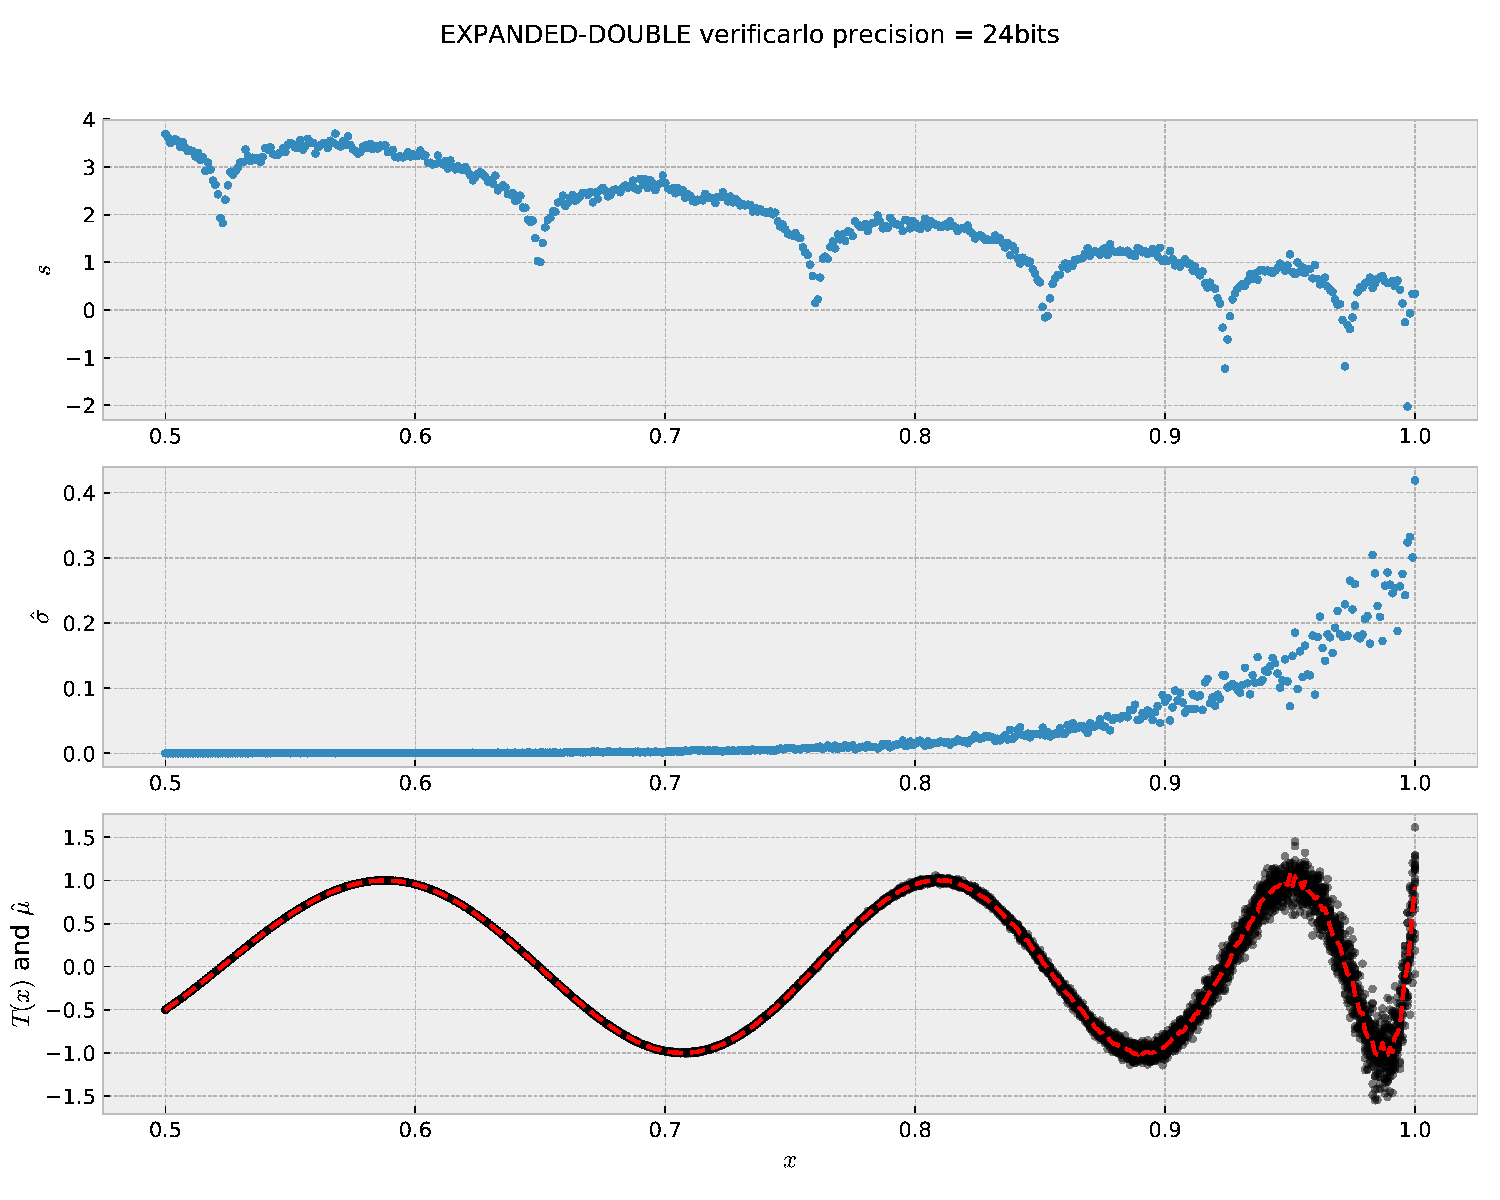
\includegraphics[width=.8\textwidth]{EXPANDED-DOUBLE-24.pdf}
  \caption{Evaluation of T(x) in its expanded form, compiled in double precision, with a virtual precision of 24}
  \label{fig:expanded:double:24}
\end{figure}
\begin{figure}[h]
\center 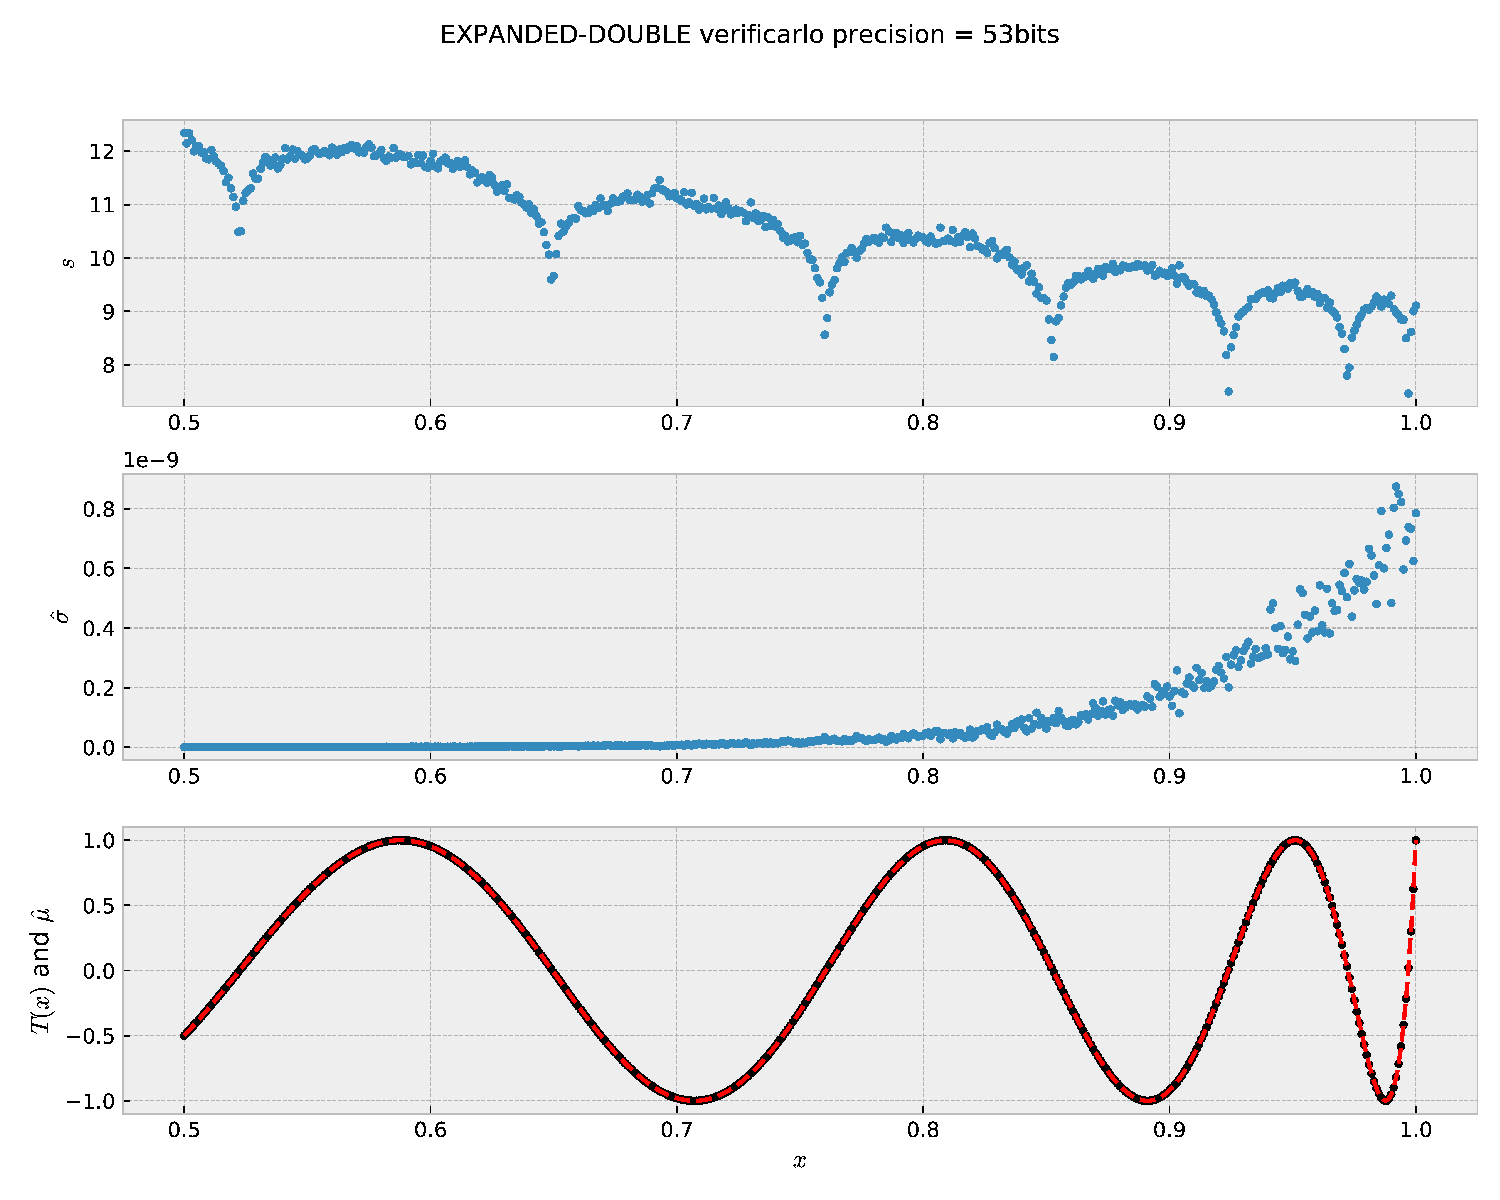
\includegraphics[width=.8\textwidth]{EXPANDED-DOUBLE-53.pdf}
  \caption{Evaluation of T(x) in its expanded form, compiled in double precision, with a virtual precision of 53}
  \label{fig:expanded:double:53}
\end{figure}

Close to 1, the polynomial evaluation is subject to {\it cancellations} which rapidly decrease the result precision. The double precision on the contrary seems satisfactory.

However using double precision is just moving the problem closer to 1 and it forces the programmer to use a larger and more costly data type.

Nevertheless if the user is already using double precision number, and if the precision is still not satisfactory, how to solve the issue? Or what if we need to use single precision?

\FloatBarrier

\subsection{Evaluation using Horner scheme}

It exists many other ways to evaluate polynomials, using associativity, commutativity and factorization. More often they are explored for sake of performance, but they also greatly influence the precision of the evaluation. One of them reputed to both performance with good numerical behavior is the Horner scheme which for our polynomial correspond to the following form:
% Horner reputed for good numerical behavior?

\[
	T(x) = (\dots((a_n\times x^2 + a_{n-1})\times x^2 + a_{n-2})\dots) \times x^2
    + a_0
\]

$$T(x) = (((((((((524288*x^2-2621440)*x^2+5570560)*x^2-6553600)*$$
$$x^2+4659200)*x^2-2050048)*x^2+549120)*x^2-84480)*$$
$$x^2+6600)*x^2-200)*x^2+1$$

\begin{question}
  \begin{enumerate}[(a)]
  \item Open the file {\tt tchebychev.c} and have a look to the function {\tt REAL horner(REAL x)}
\item While keeping previous execution parameters, execute the command {\tt ./run.sh HORNER DOUBLE 53}.  \newline The output of this command is given in figure~\ref{fig:horner:double:53}.
  \end{enumerate}
\end{question}

\begin{question}
 \item Modify the {\tt run.sh} script to evaluate the polynomial from $0.5$ to $1$ by $0.001$.
\item Execute the command {\tt ./run.sh HORNER DOUBLE 24}  \newline
The output of this command is given in figure~\ref{fig:horner:double:24}.

\end{question}

As shown in this experiment, the Horner scheme has a limited influence on the result precision ($\simeq$ 1 more bit). However, it minimizes the number of operations and allows to use the FMA ({\it Fused Multiply Add}). For a polynomial of degree $n$, it produces $n-1$ FMA. Moreover, when doing multiple independent evaluations it can be vectorized.


\begin{figure}[htb]
\center 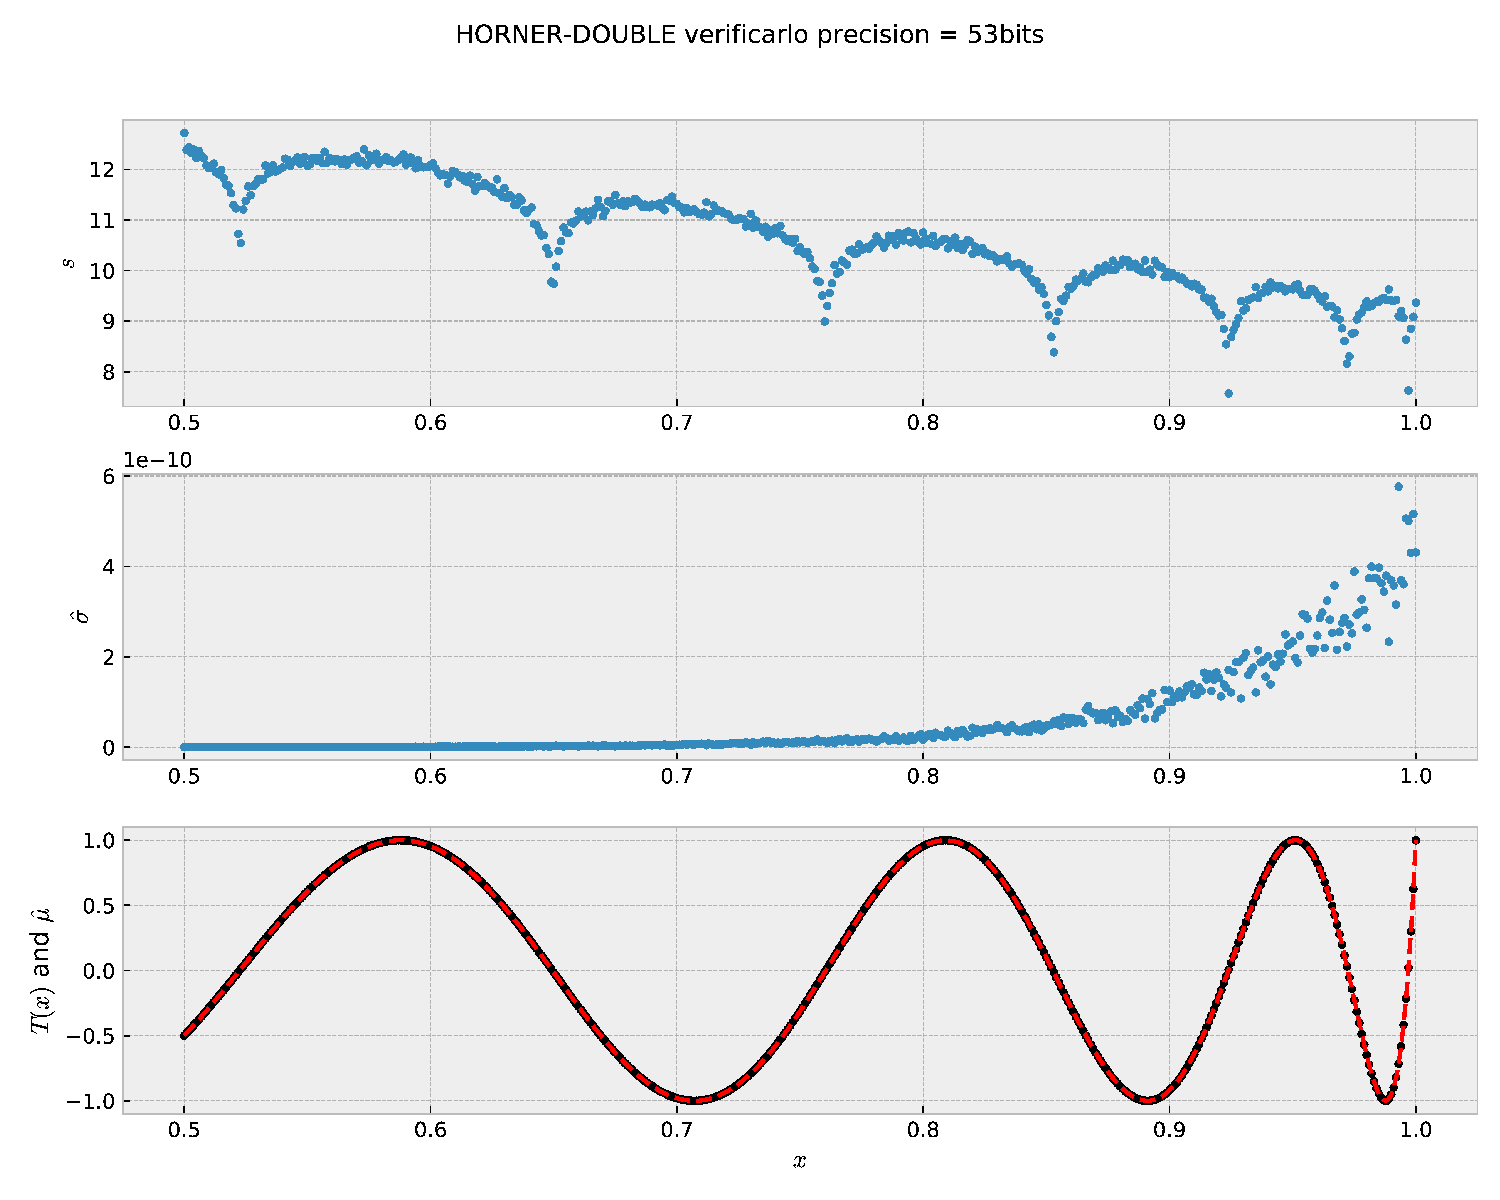
\includegraphics[width=.8\textwidth]{HORNER-DOUBLE-53.pdf}
  \caption{Evaluation of T(x) using Horner scheme, compiled in double precision, with a virtual precision of 53}
  \label{fig:horner:double:53}
\end{figure}
\begin{figure}[htb]
\center 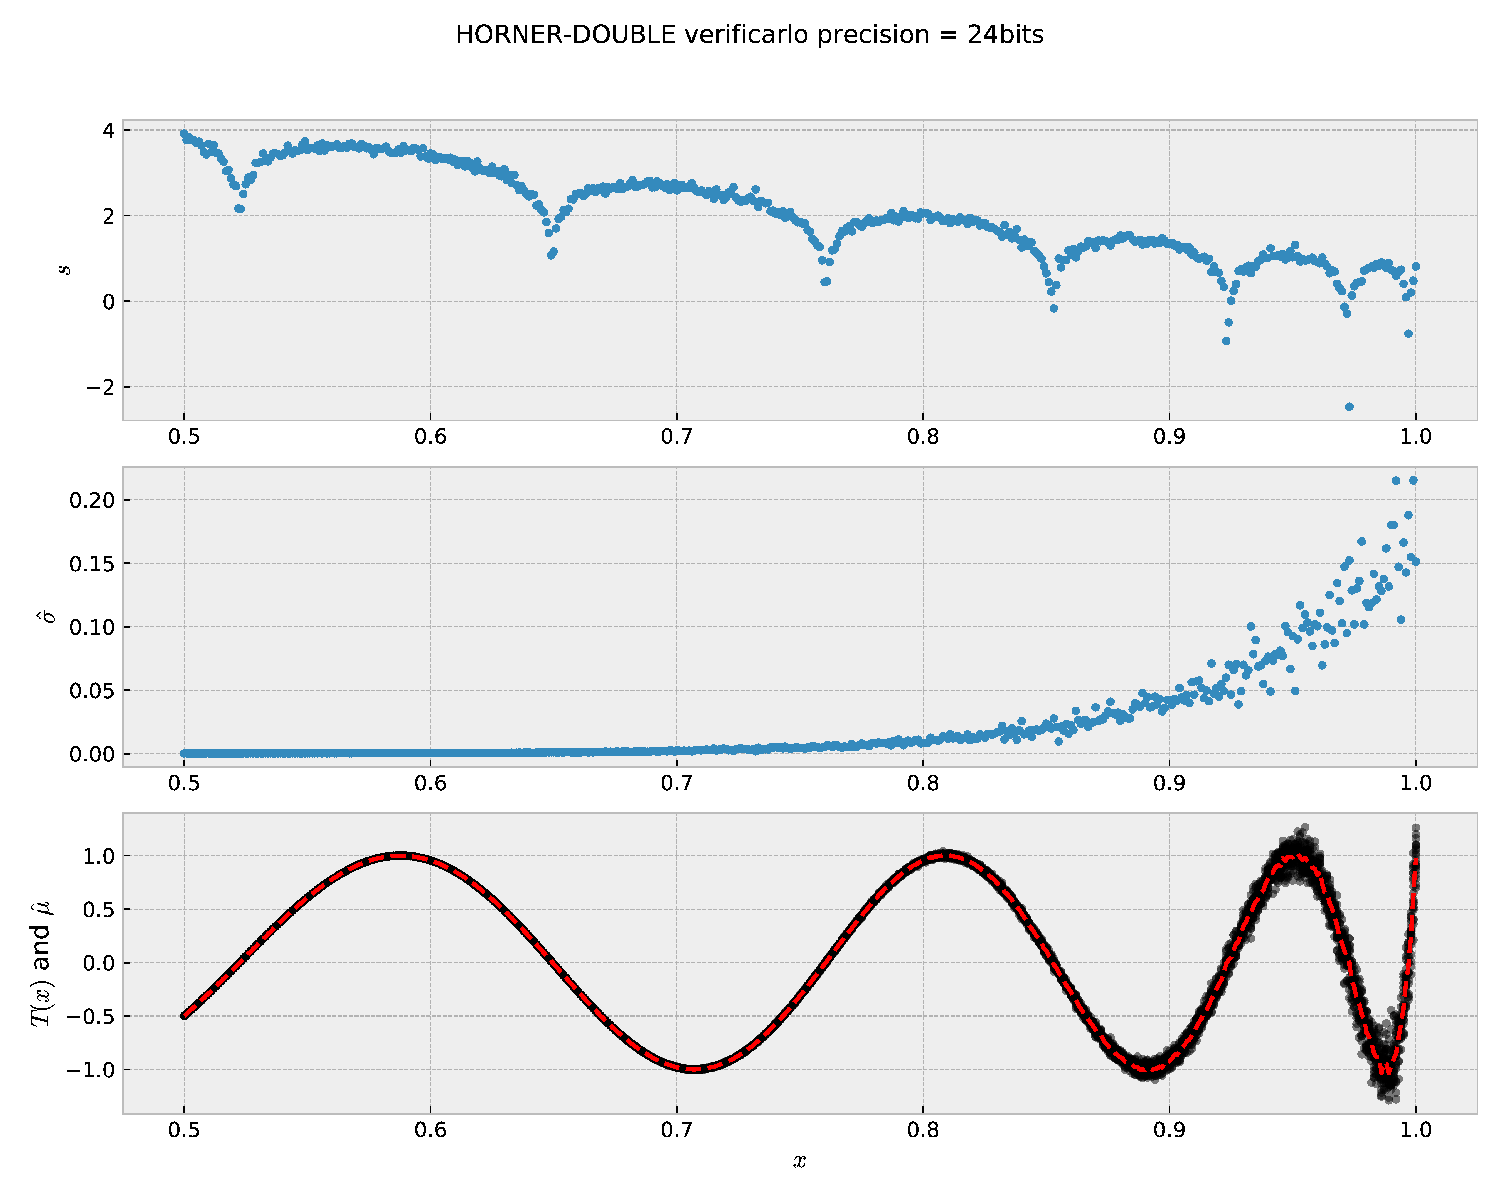
\includegraphics[width=.8\textwidth]{HORNER-DOUBLE-24.pdf}
  \caption{Evaluation of T(x) using Horner scheme, compiled in double precision, with a virtual precision of 24}
  \label{fig:horner:double:24}
\end{figure}


\FloatBarrier

\subsection{Factored form}

We will now evaluate the evaluation precision of the following factored rewriting:
\[
	T(x) = 1 + 8x^2\,(x-1)\,(x+1)\,(4x^2 + 2x - 1)^2\, (4x^2 - 2x - 1)^2\,(16x^4 - 20x^2 + 5)^2
\]

\begin{eqnarray*}
T(x) &=& 8.0*x^2*(x - 1.0)*(x + 1.0) \\
 & & * (4.0*x^2 + 2.0*x - 1.0)*(4.0*x^2 + 2.0*x - 1.0) \\
 & & * (4.0*x^2 - 2.0*x - 1.0)*(4.0*x^2 - 2.0*x - 1.0)* \\
 & & * (16.0*x^4 - 20.0*x^2 + 5.0)*(16.0*x^4 - 20.0*x^2 + 5.0) + 1 \\
\end{eqnarray*}

\begin{question}
  \begin{enumerate}[(a)]
  \item Open the file {\tt tchebychev.c} and have a look to the function {\tt REAL factored (REAL x)}
\item Execute the command {\tt ./run.sh FACTORED DOUBLE 24} \newline
The output of this command is given in figure~\ref{fig:factored:double:24}.
\item Compare these results to those obtained with EXPANDED and HORNER versions.
  \end{enumerate}
\end{question}

\begin{figure}[h]
\center 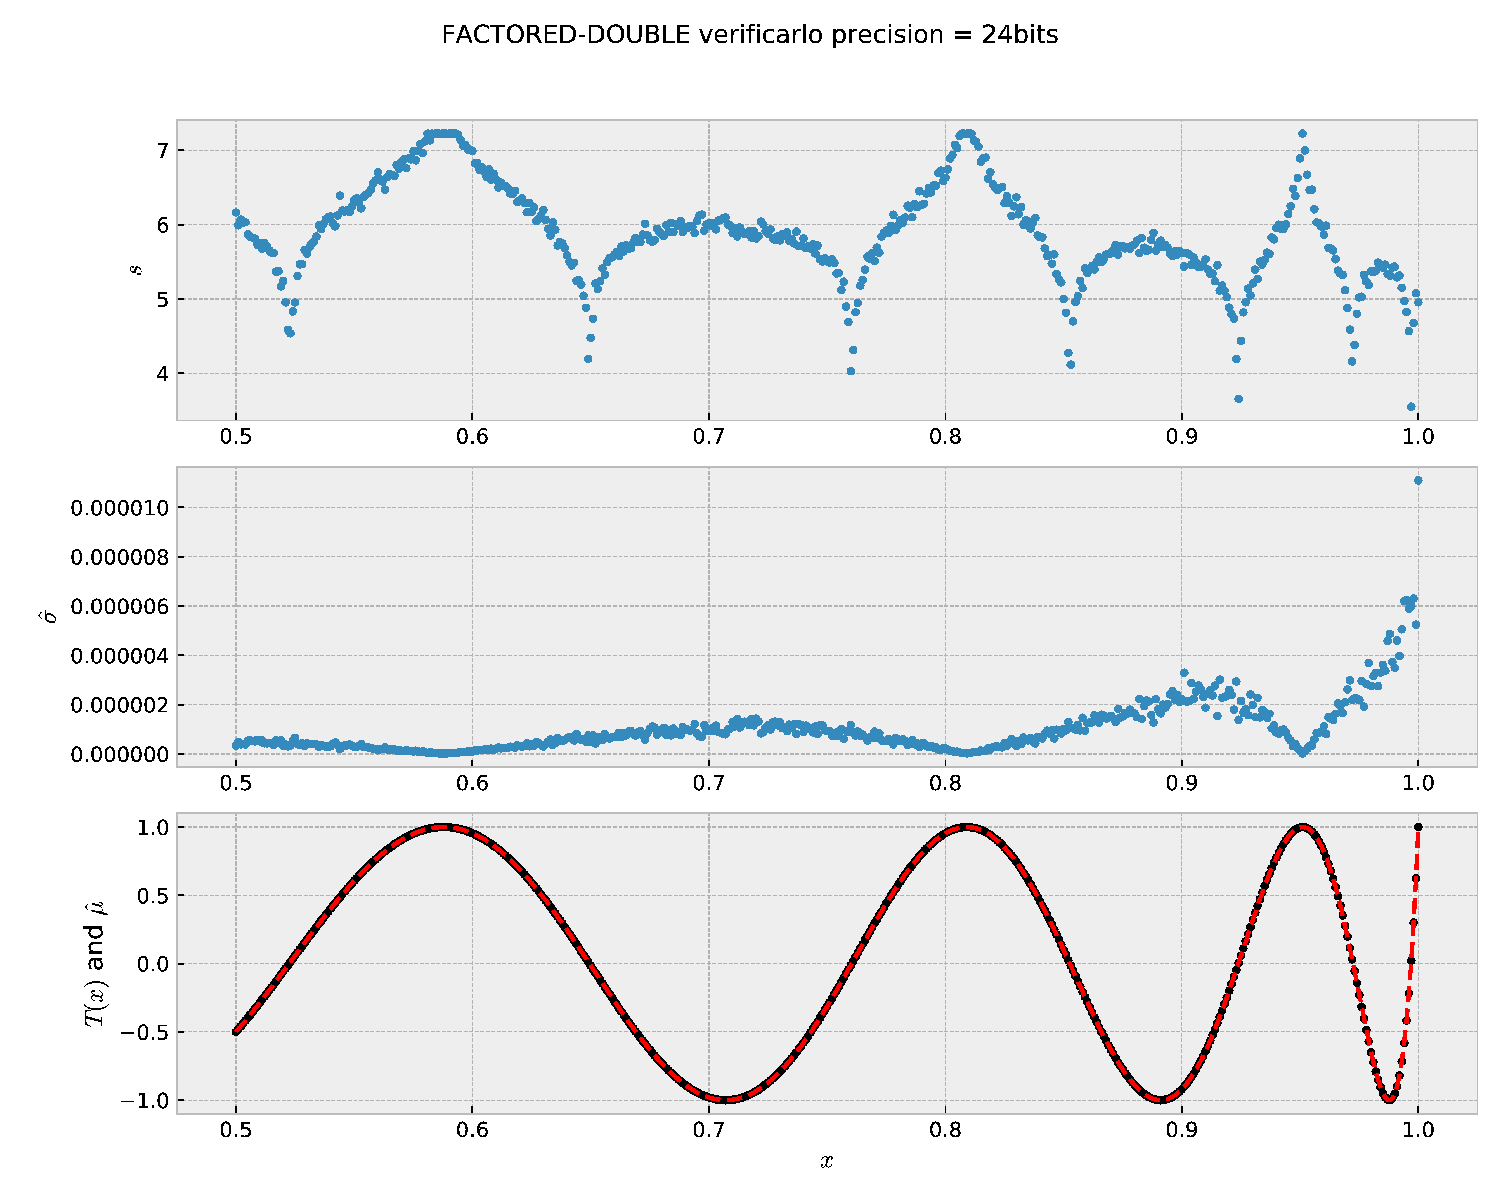
\includegraphics[width=.8\textwidth]{FACTORED-DOUBLE-24.pdf}
  \caption{Evaluation of T(x) in its factored form, compiled in double precision, with a virtual precision of 24}
  \label{fig:factored:double:24}
\end{figure}

\begin{question}
  Explain what happens when $T(x)=1$ for $x\simeq 0.6$,
  $x\simeq 0.8$ et $x\simeq 0.95$.\\~\\
  $\rightarrow$ It is an example where the error is absorbed and the precision and accuracy  of the results are improved.
\end{question}


\begin{question}
  \begin{enumerate}[(a)]
    \item Modify the {\tt run.sh} script to evaluate the  polynomial between $0.99$ and $1$ by $0.00001$ step.
  \item Run the scripts to execute and visualize the results for
    FACTORED, EXPANDED and HORNER with a virtual precision of 53. The results are respectively presented in figure~\ref{fig:factored:double:53:zoom},\ref{fig:expanded:double:53:zoom}
    and~\ref{fig:horner:double:53:zoom}.

\item Reproduce the result with a virtual precision of 24. The results are respectively presented in figure~\ref{fig:factored:double:24:zoom},\ref{fig:expanded:double:24:zoom}
    and~\ref{fig:horner:double:24:zoom}

\end{enumerate}
\end{question}

\begin{figure}[h]
  \center 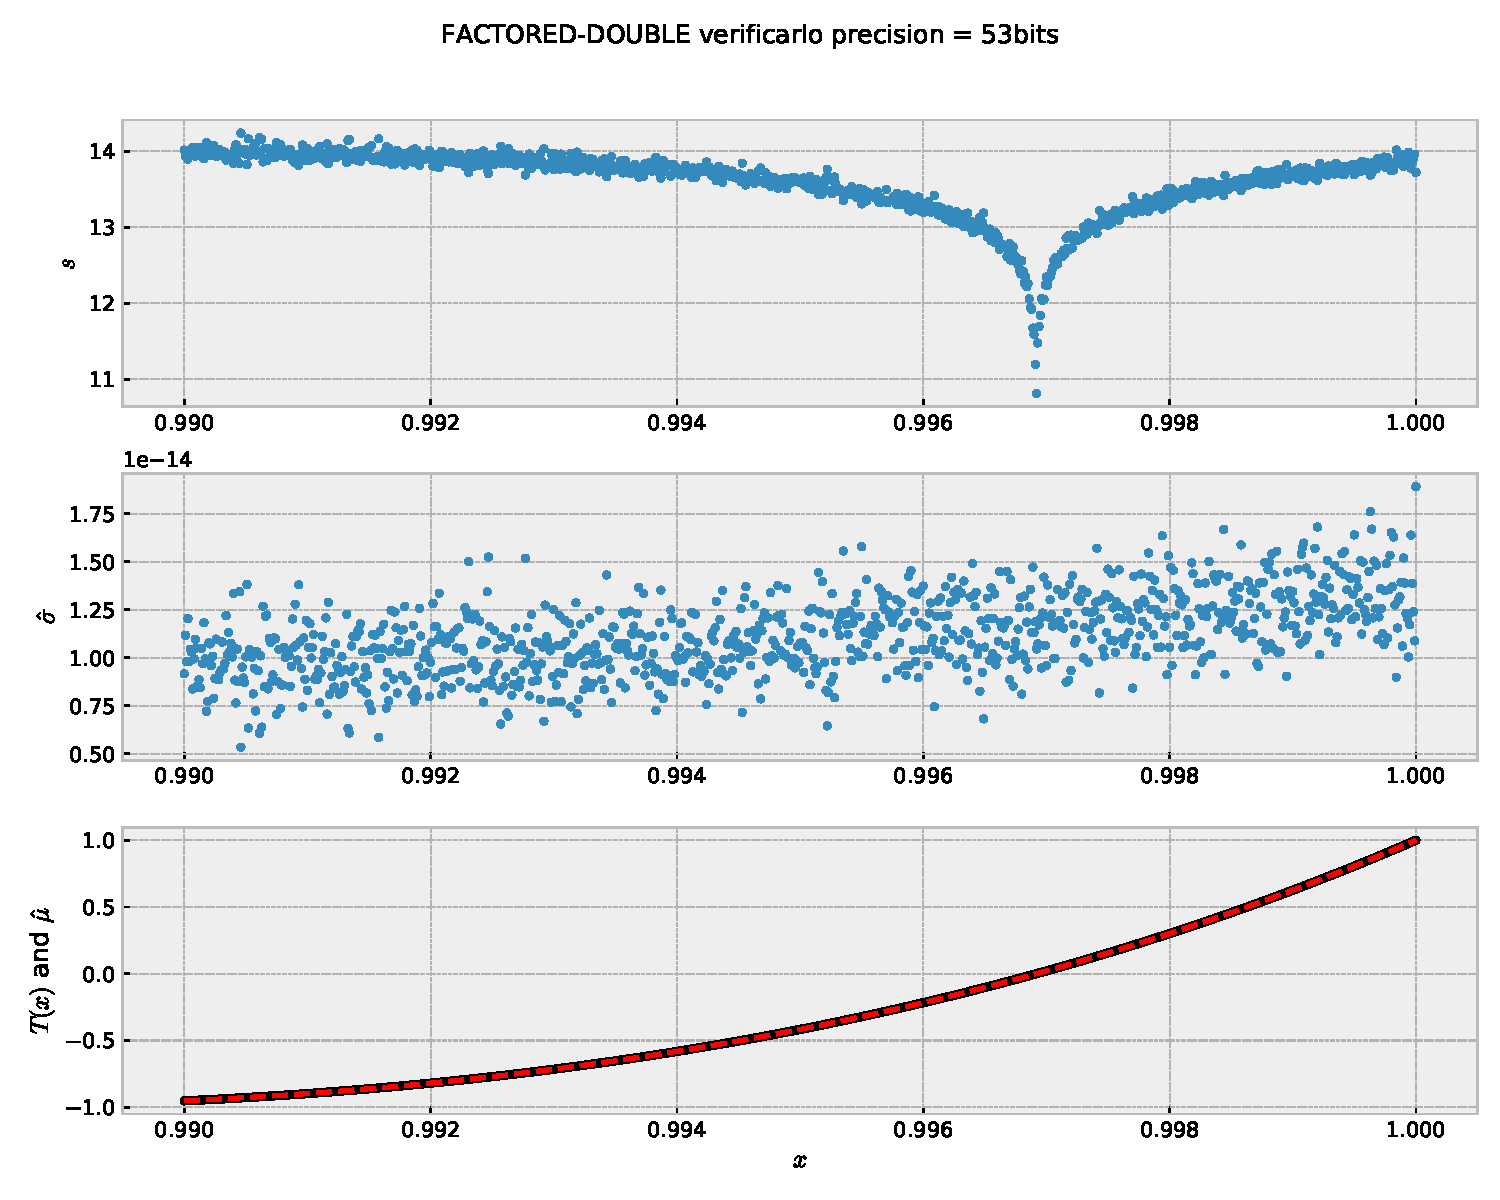
\includegraphics[width=.8\textwidth]{FACTORED-DOUBLE-53-zoom.pdf}
  \caption{Evaluation of T(x) in its factored form, compiled in double
    precision, with a virtual precision of 53}
  \label{fig:factored:double:53:zoom}
\end{figure}

\begin{figure}[h]
  \center 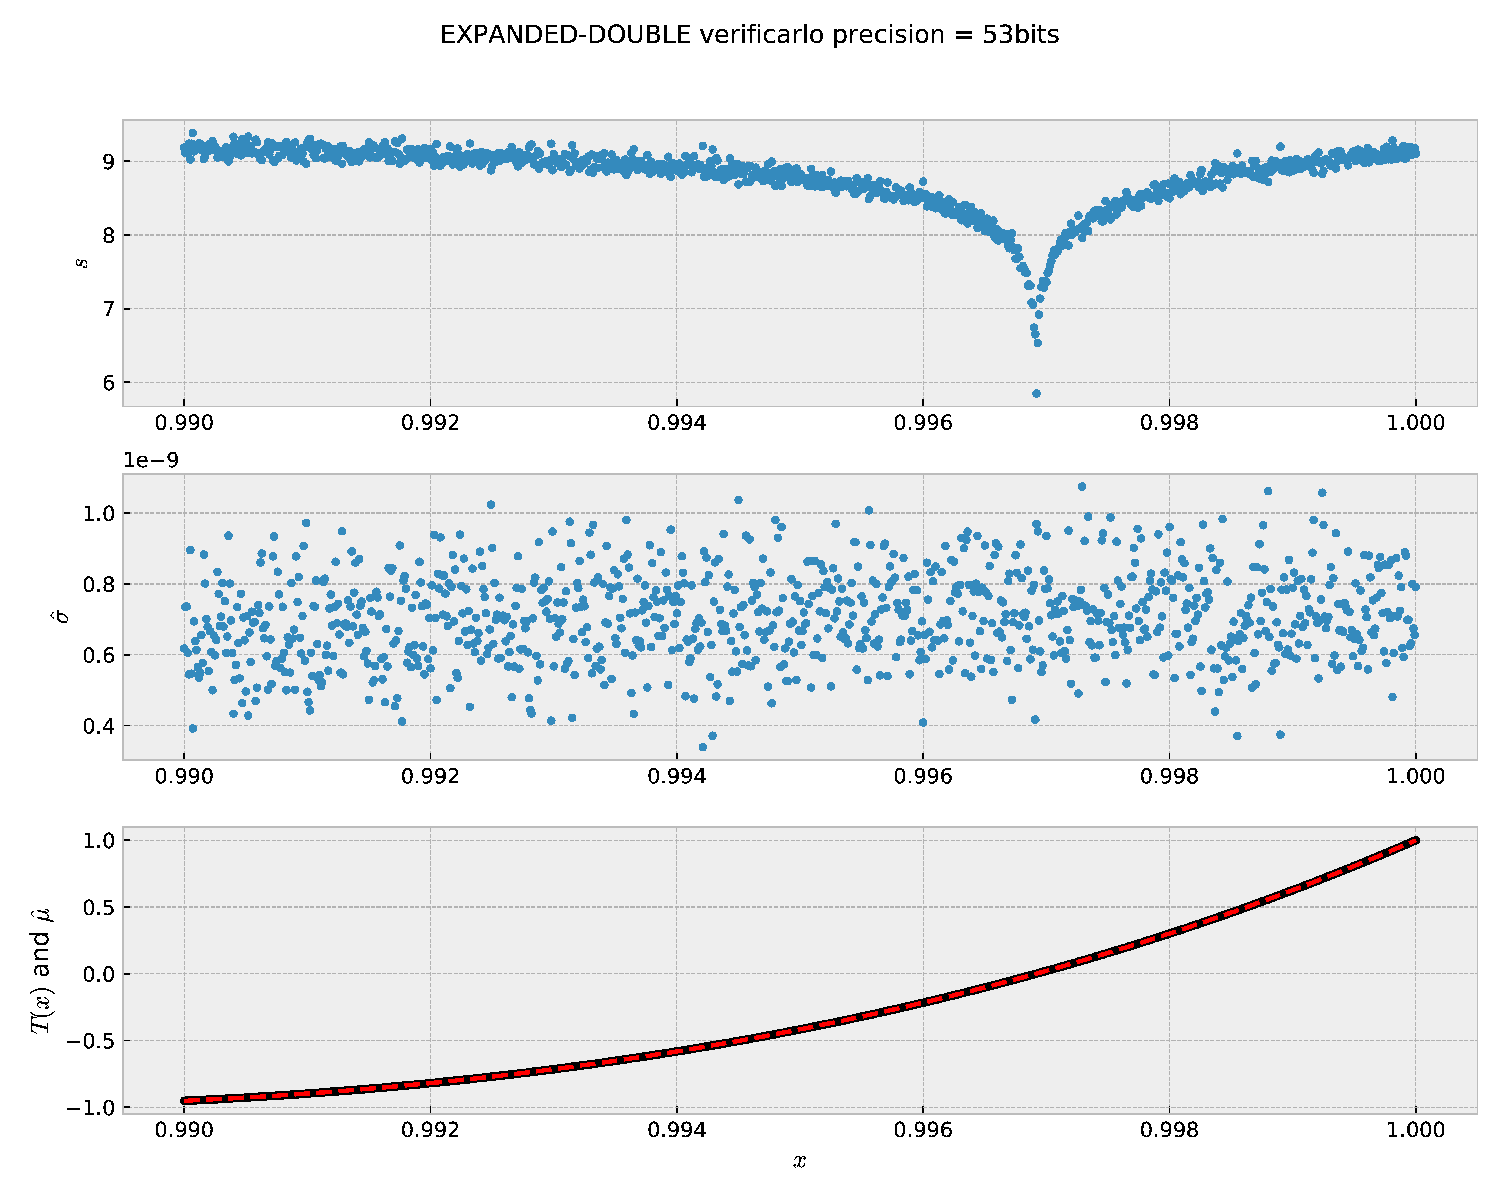
\includegraphics[width=.8\textwidth]{EXPANDED-DOUBLE-53-zoom.pdf}
  \caption{Evaluation of T(x) in its expanded form, compiled in double
    precision, with a virtual precision of 53}
  \label{fig:expanded:double:53:zoom}
\end{figure}

\begin{figure}[h]
  \center 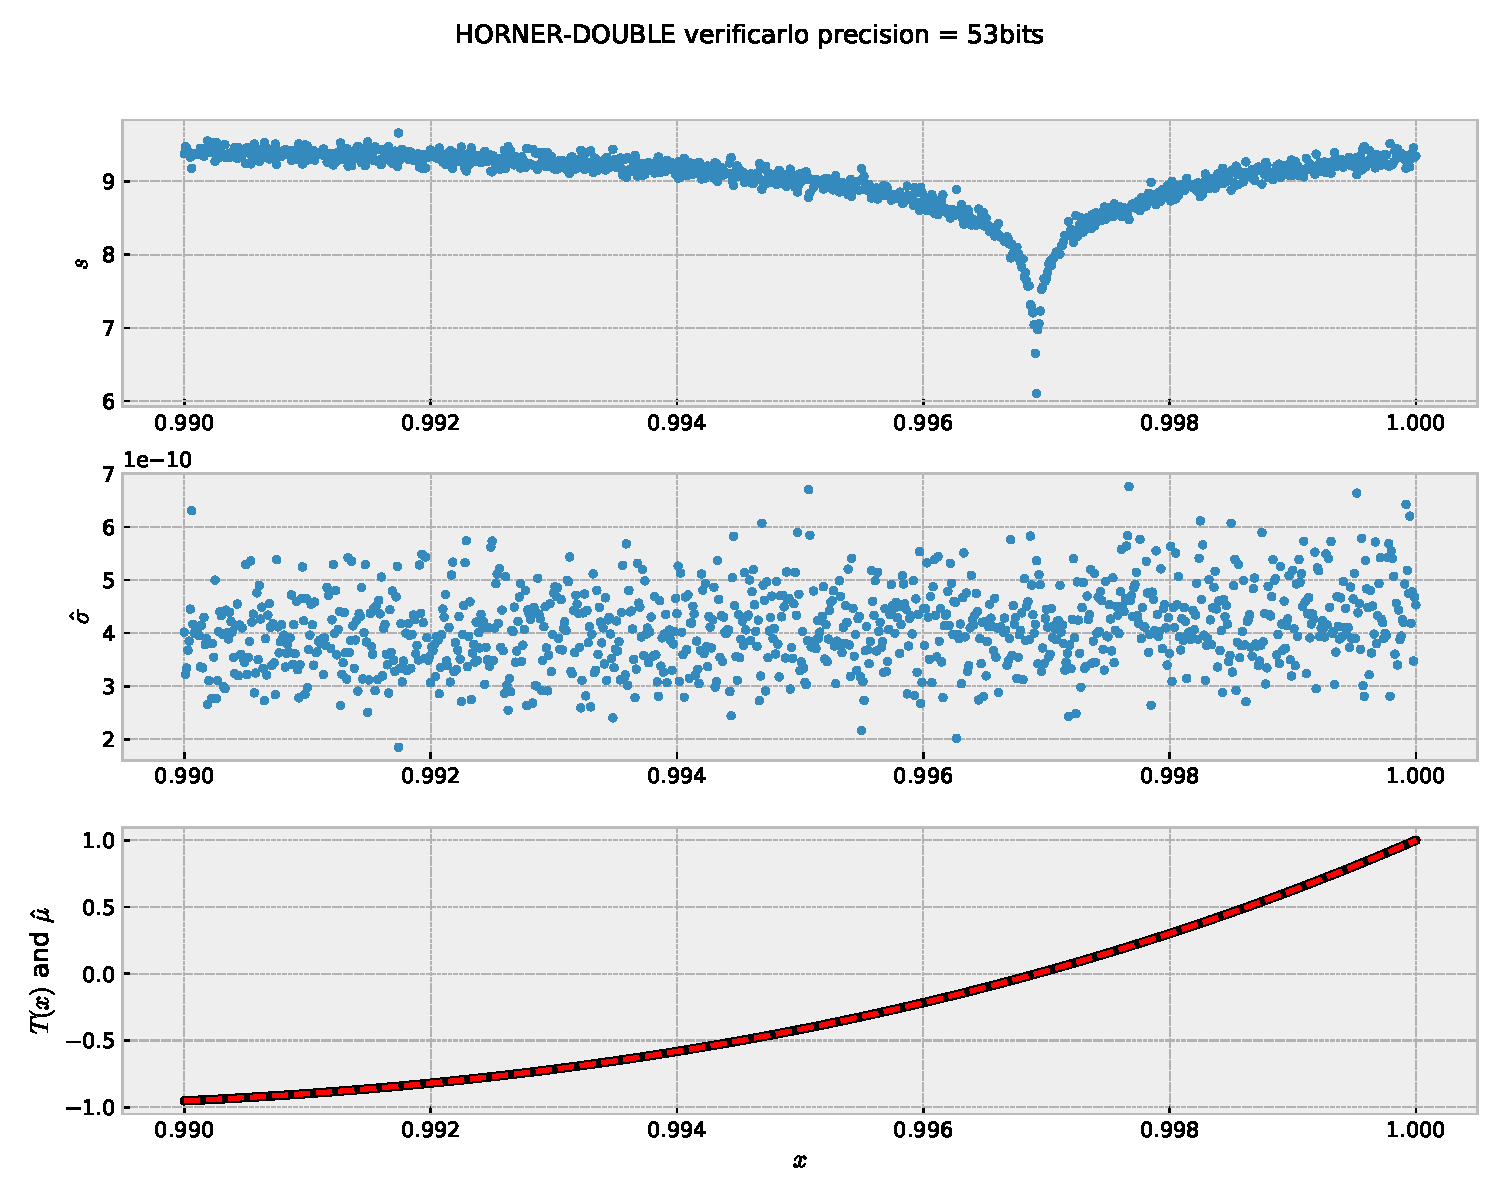
\includegraphics[width=.8\textwidth]{HORNER-DOUBLE-53-zoom.pdf}
  \caption{Evaluation of T(x) using Horner scheme, compiled in double precision,
    with a virtual precision of 53}
  \label{fig:horner:double:53:zoom}
\end{figure}

\begin{figure}[h]
  \center 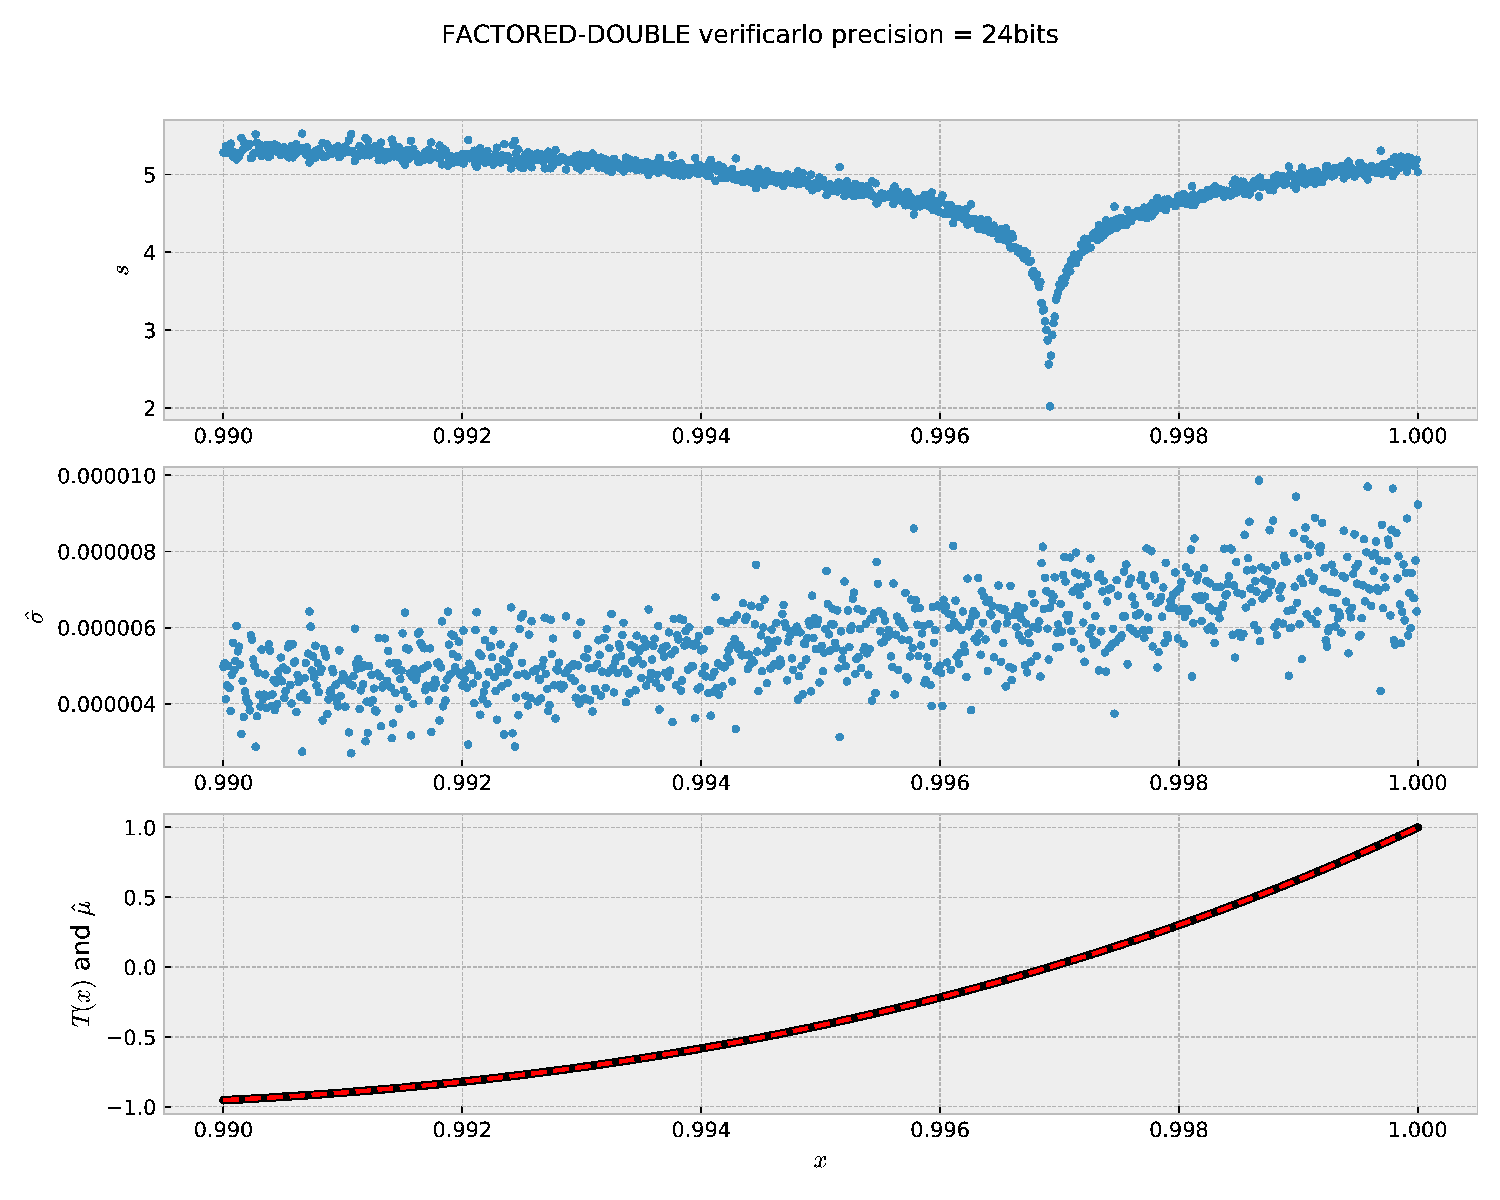
\includegraphics[width=.8\textwidth]{FACTORED-DOUBLE-24-zoom.pdf}
  \caption{Evaluation of T(x) in its factored form, compiled in double
    precision, with a virtual precision of 24}
  \label{fig:factored:double:24:zoom}
\end{figure}

\begin{figure}[h]
  \center 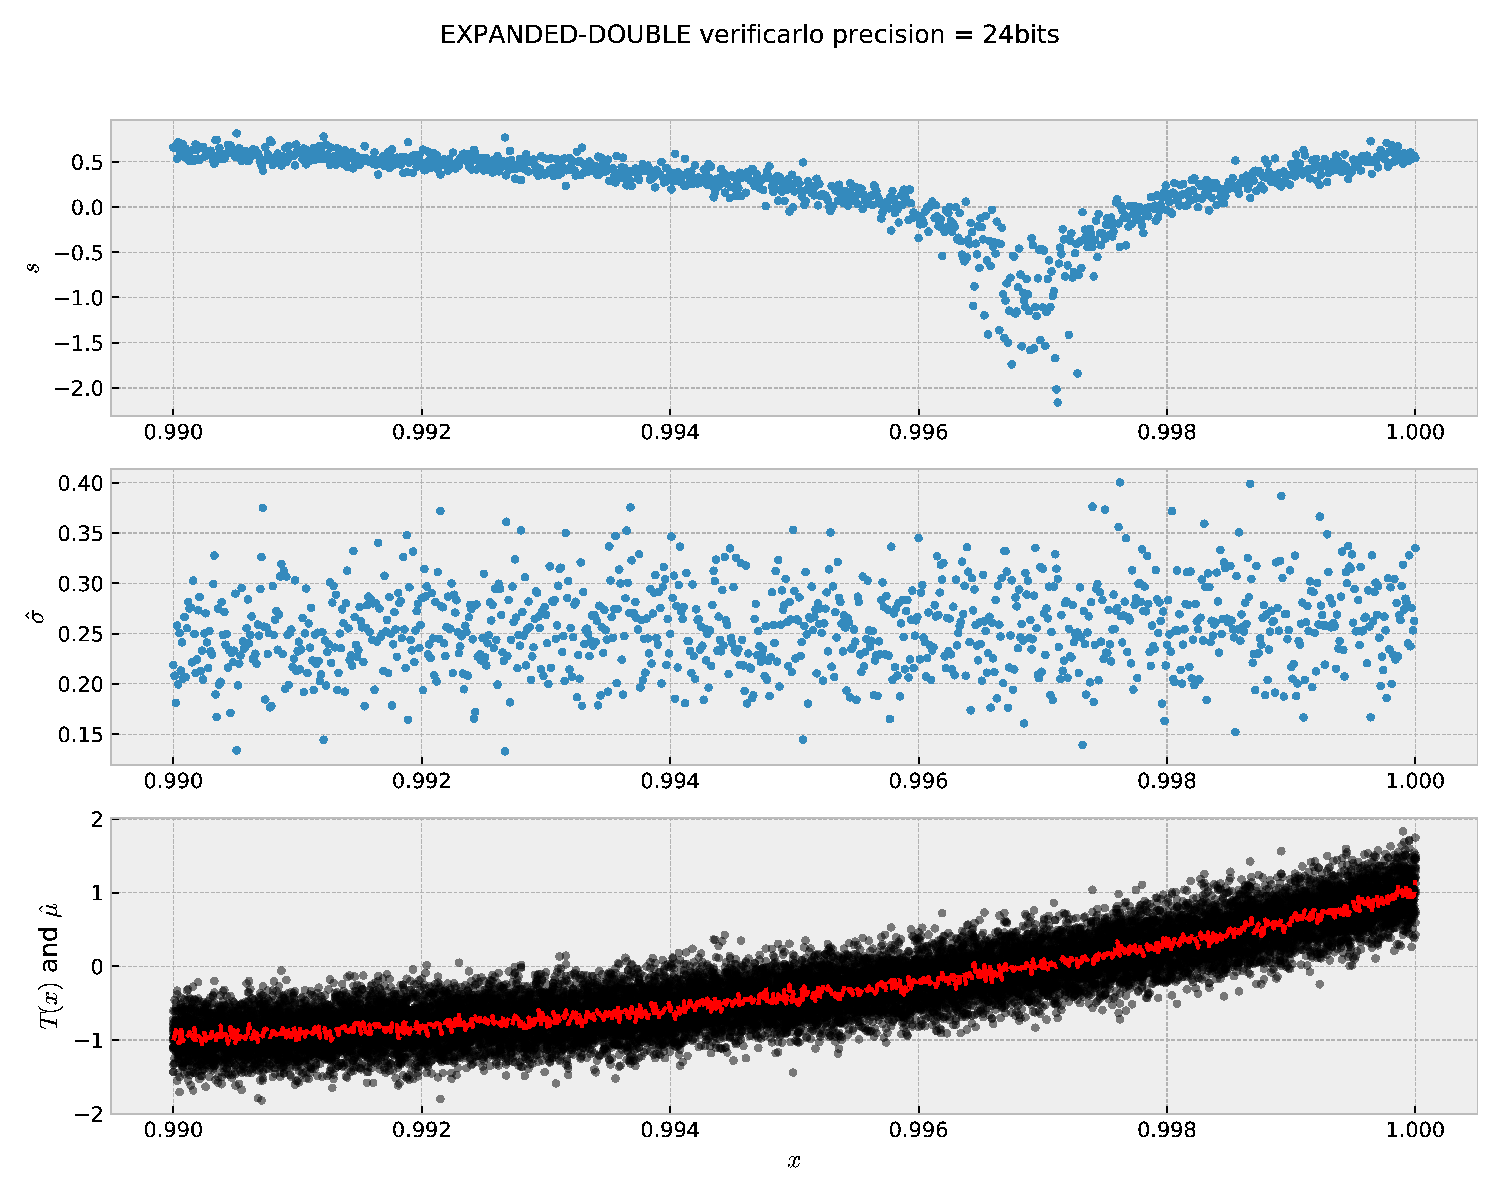
\includegraphics[width=.8\textwidth]{EXPANDED-DOUBLE-24-zoom.pdf}
  \caption{Evaluation of T(x) in its expanded form, compiled in double
    precision, with a virtual precision of 24}
  \label{fig:expanded:double:24:zoom}
\end{figure}

\begin{figure}[h]
  \center 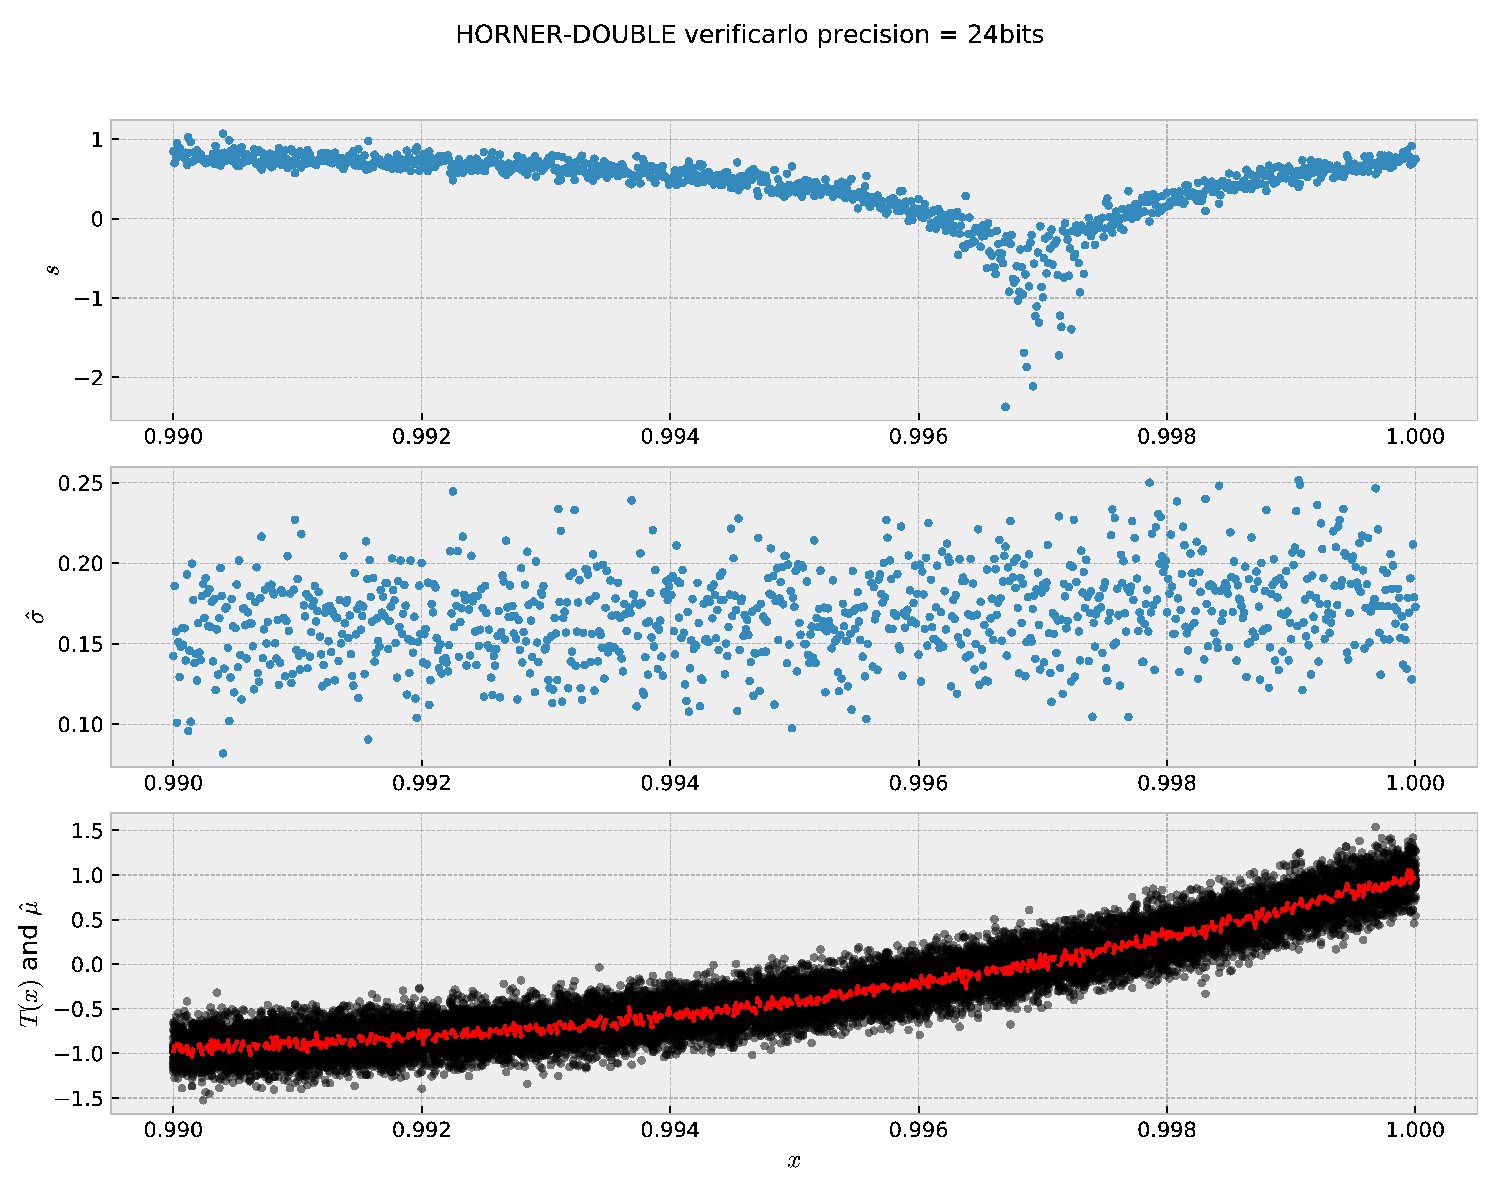
\includegraphics[width=.8\textwidth]{HORNER-DOUBLE-24-zoom.pdf}
  \caption{Evaluation of T(x) using Horner scheme, compiled in double precision,
    with a virtual precision of 24}
    \label{fig:horner:double:24:zoom}
\end{figure}

\subsection{Conclusion}


From a general stand point, for every arithmetic expression in a program, it exists many valid rewriting. They are not all equivalent in terms of performance, precision, and accuracy!

\begin{question}
What is the best approach?
\end{question}

\FloatBarrier



%% Uncomment below lines to include the extra Factored Form analysis
%% \FloatBarrier
%% \subsection{Factored form}

We will now evaluate the evaluation precision of the following factored rewriting:
\[
	T(x) = 1 + 8x^2\,(x-1)\,(x+1)\,(4x^2 + 2x - 1)^2\, (4x^2 - 2x - 1)^2\,(16x^4 - 20x^2 + 5)^2
\]

\begin{eqnarray*}
T(x) &=& 8.0*x^2*(x - 1.0)*(x + 1.0) \\
 & & * (4.0*x^2 + 2.0*x - 1.0)*(4.0*x^2 + 2.0*x - 1.0) \\
 & & * (4.0*x^2 - 2.0*x - 1.0)*(4.0*x^2 - 2.0*x - 1.0)* \\
 & & * (16.0*x^4 - 20.0*x^2 + 5.0)*(16.0*x^4 - 20.0*x^2 + 5.0) + 1 \\
\end{eqnarray*}

\begin{question}
  \begin{enumerate}[(a)]
  \item Open the file {\tt tchebychev.c} and have a look to the function {\tt REAL factored (REAL x)}
\item Execute the command {\tt ./run.sh FACTORED DOUBLE 24} \newline
The output of this command is given in figure~\ref{fig:factored:double:24}.
\item Compare these results to those obtained with EXPANDED and HORNER versions.
  \end{enumerate}
\end{question}

\begin{figure}[h]
\center 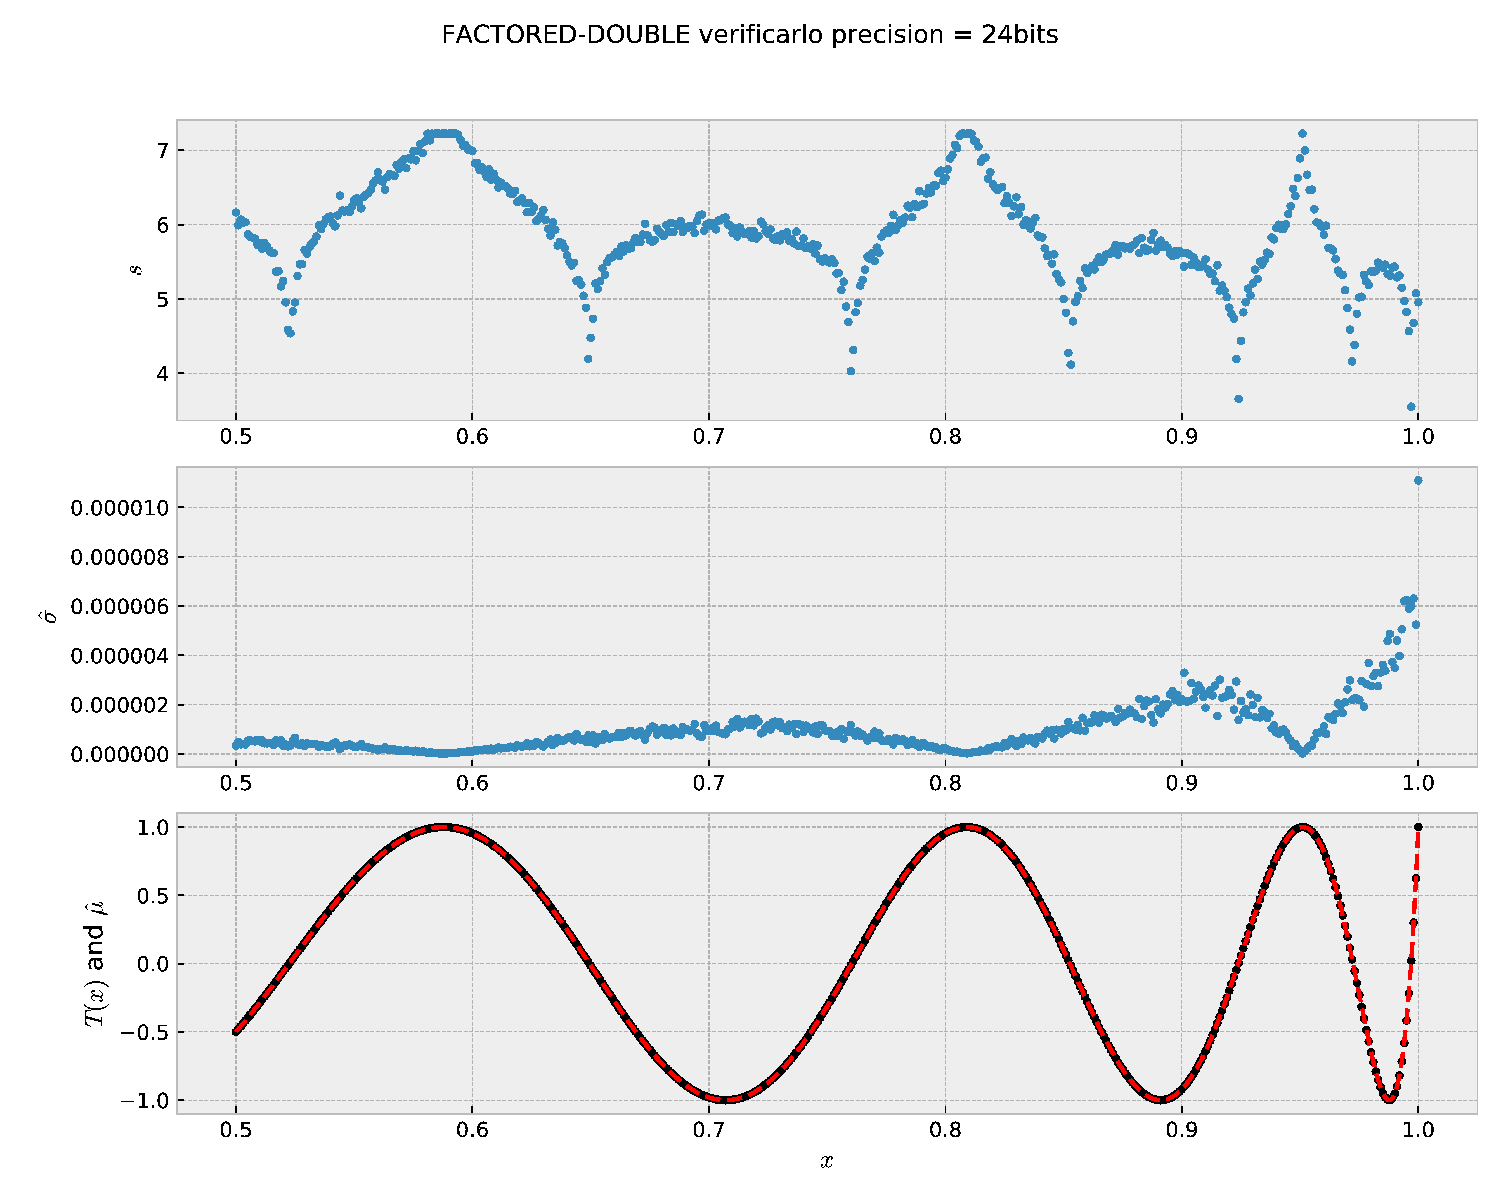
\includegraphics[width=.8\textwidth]{FACTORED-DOUBLE-24.pdf}
  \caption{Evaluation of T(x) in its factored form, compiled in double precision, with a virtual precision of 24}
  \label{fig:factored:double:24}
\end{figure}

\begin{question}
  Explain what happens when $T(x)=1$ for $x\simeq 0.6$,
  $x\simeq 0.8$ et $x\simeq 0.95$.\\~\\
  $\rightarrow$ It is an example where the error is absorbed and the precision and accuracy  of the results are improved.
\end{question}


\begin{question}
  \begin{enumerate}[(a)]
    \item Modify the {\tt run.sh} script to evaluate the  polynomial between $0.99$ and $1$ by $0.00001$ step.
  \item Run the scripts to execute and visualize the results for
    FACTORED, EXPANDED and HORNER with a virtual precision of 53. The results are respectively presented in figure~\ref{fig:factored:double:53:zoom},\ref{fig:expanded:double:53:zoom}
    and~\ref{fig:horner:double:53:zoom}.

\item Reproduce the result with a virtual precision of 24. The results are respectively presented in figure~\ref{fig:factored:double:24:zoom},\ref{fig:expanded:double:24:zoom}
    and~\ref{fig:horner:double:24:zoom}

\end{enumerate}
\end{question}

\begin{figure}[h]
  \center 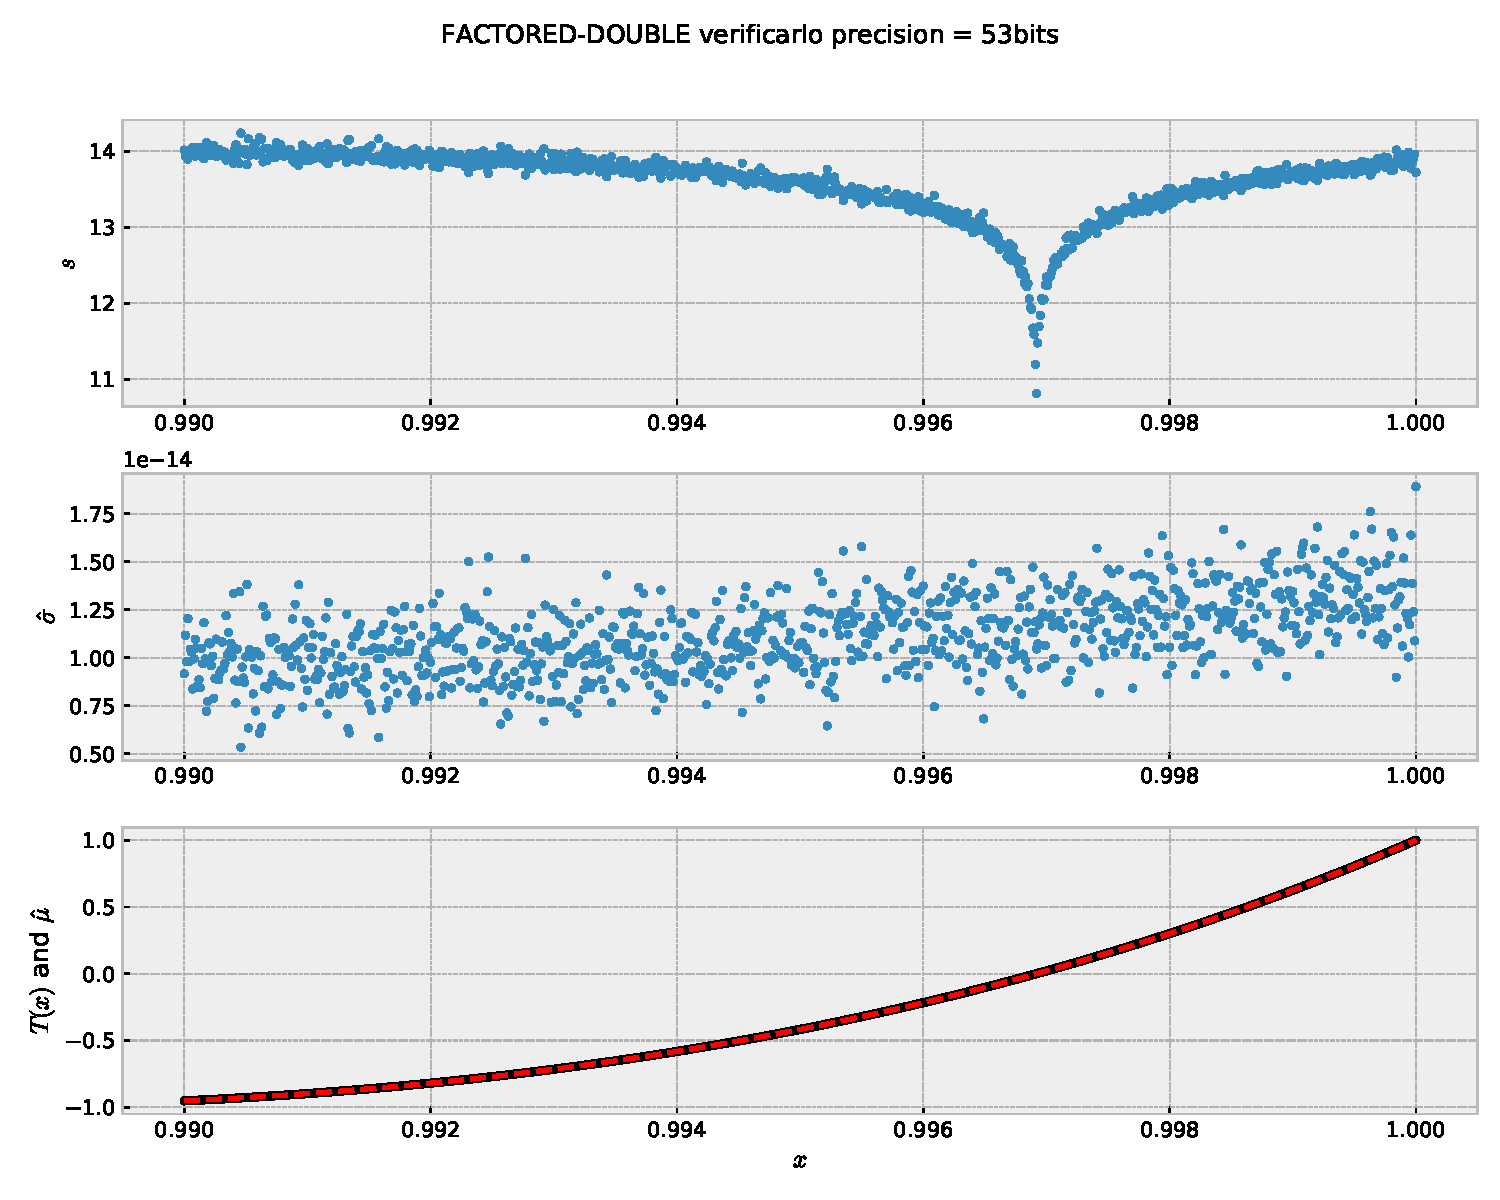
\includegraphics[width=.8\textwidth]{FACTORED-DOUBLE-53-zoom.pdf}
  \caption{Evaluation of T(x) in its factored form, compiled in double
    precision, with a virtual precision of 53}
  \label{fig:factored:double:53:zoom}
\end{figure}

\begin{figure}[h]
  \center 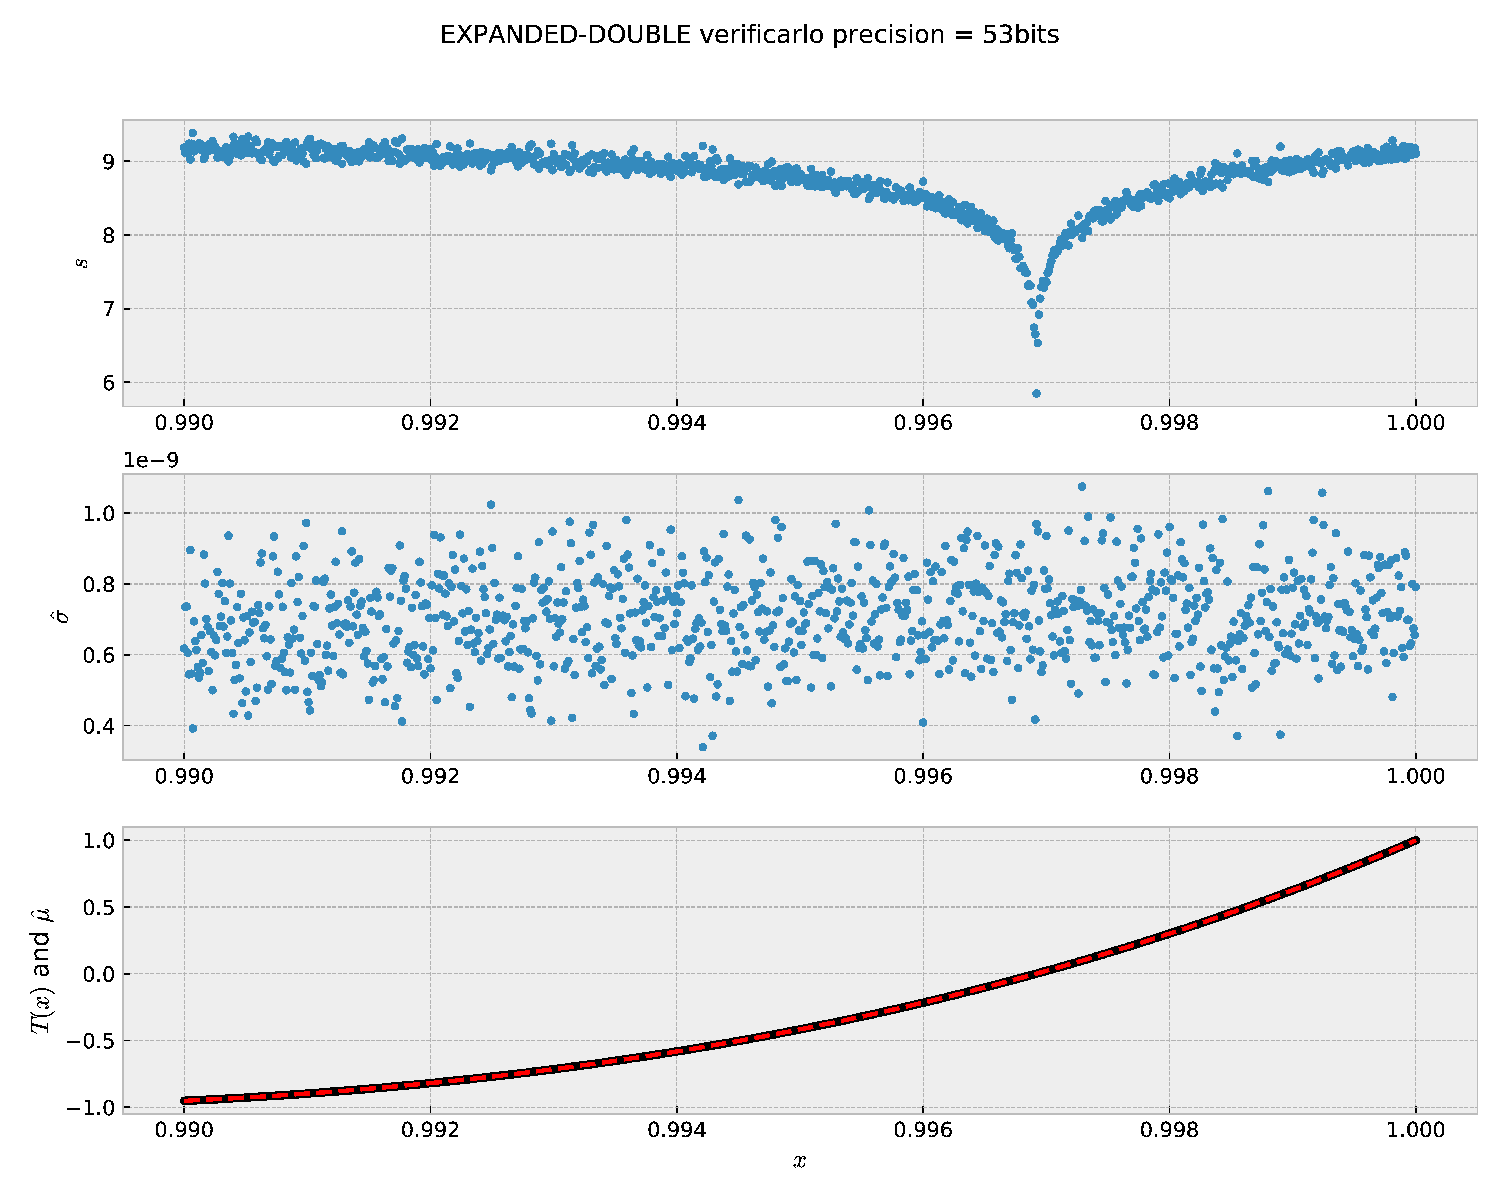
\includegraphics[width=.8\textwidth]{EXPANDED-DOUBLE-53-zoom.pdf}
  \caption{Evaluation of T(x) in its expanded form, compiled in double
    precision, with a virtual precision of 53}
  \label{fig:expanded:double:53:zoom}
\end{figure}

\begin{figure}[h]
  \center 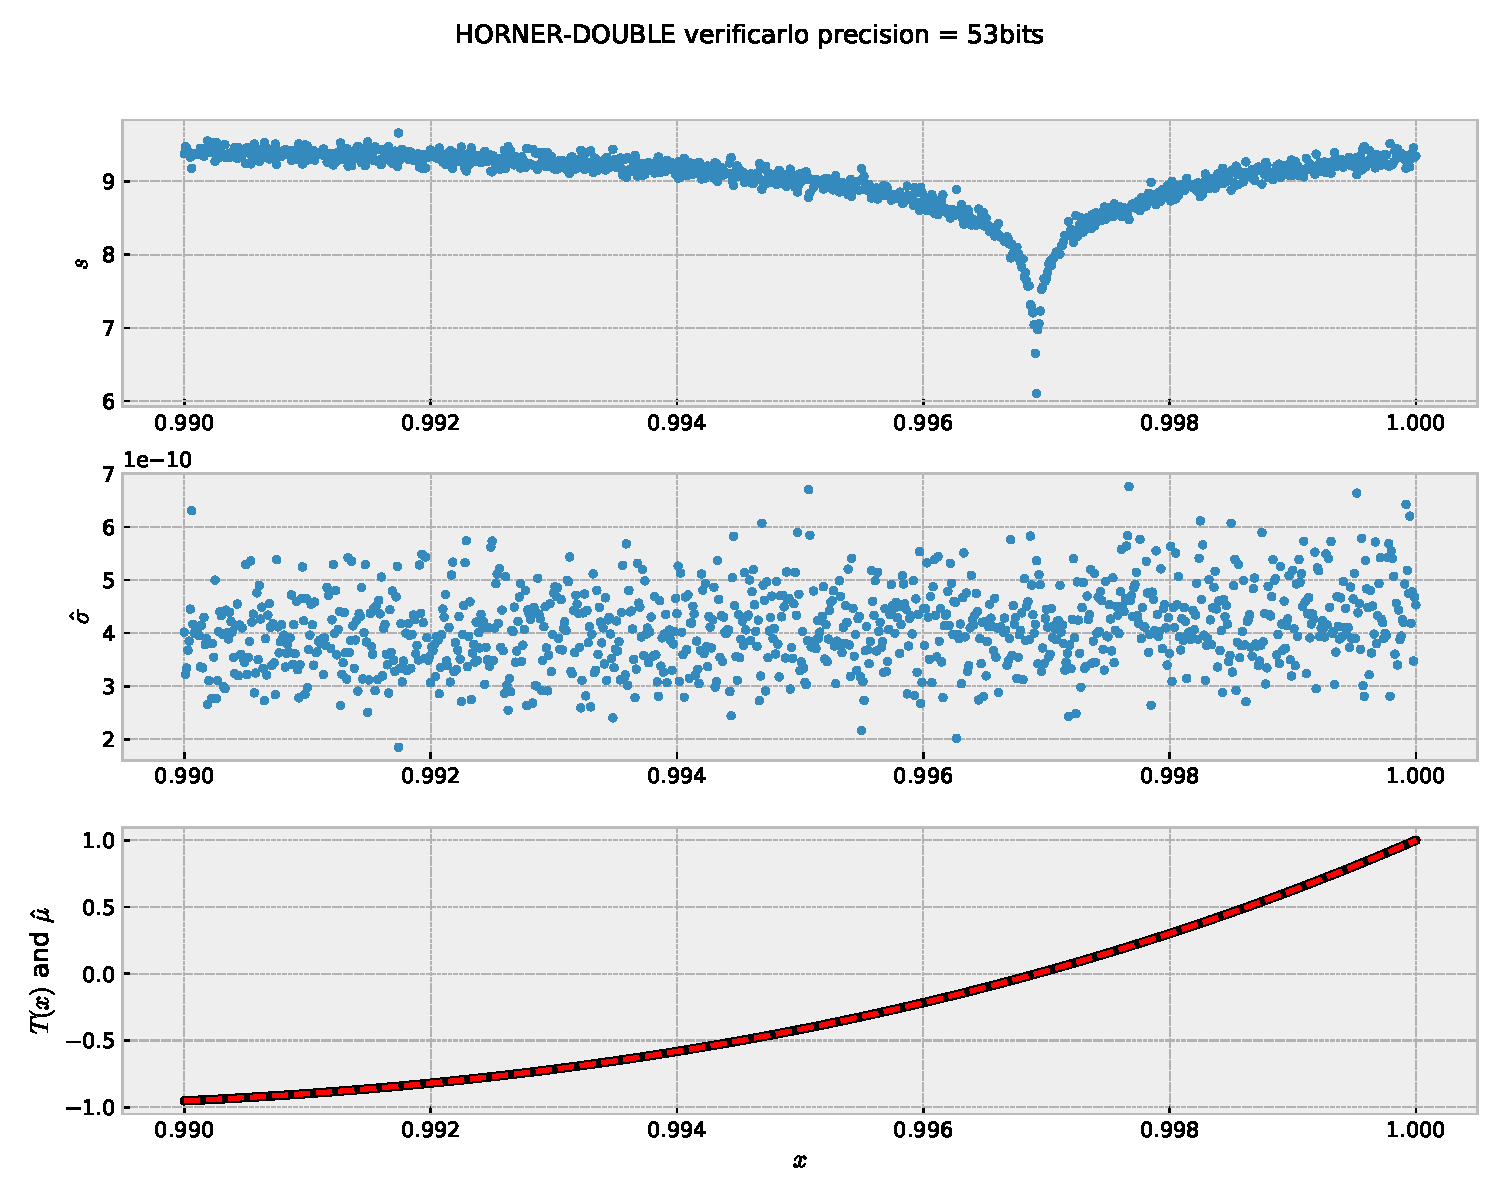
\includegraphics[width=.8\textwidth]{HORNER-DOUBLE-53-zoom.pdf}
  \caption{Evaluation of T(x) using Horner scheme, compiled in double precision,
    with a virtual precision of 53}
  \label{fig:horner:double:53:zoom}
\end{figure}

\begin{figure}[h]
  \center 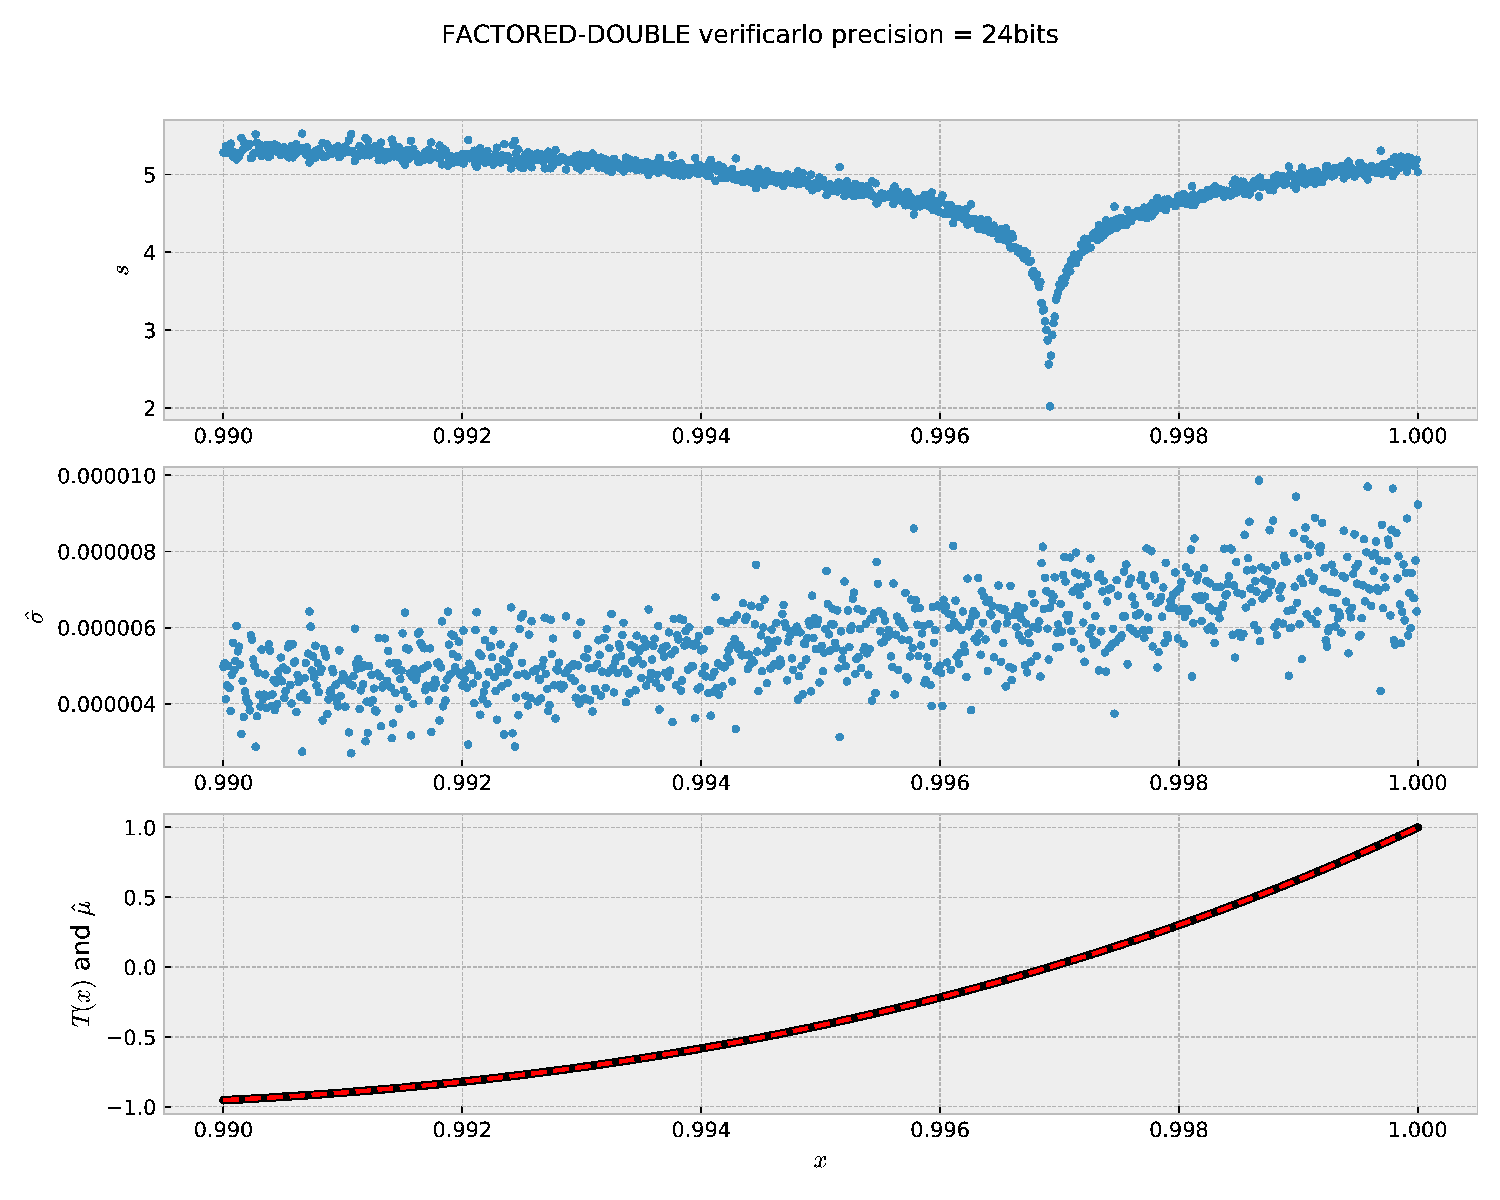
\includegraphics[width=.8\textwidth]{FACTORED-DOUBLE-24-zoom.pdf}
  \caption{Evaluation of T(x) in its factored form, compiled in double
    precision, with a virtual precision of 24}
  \label{fig:factored:double:24:zoom}
\end{figure}

\begin{figure}[h]
  \center 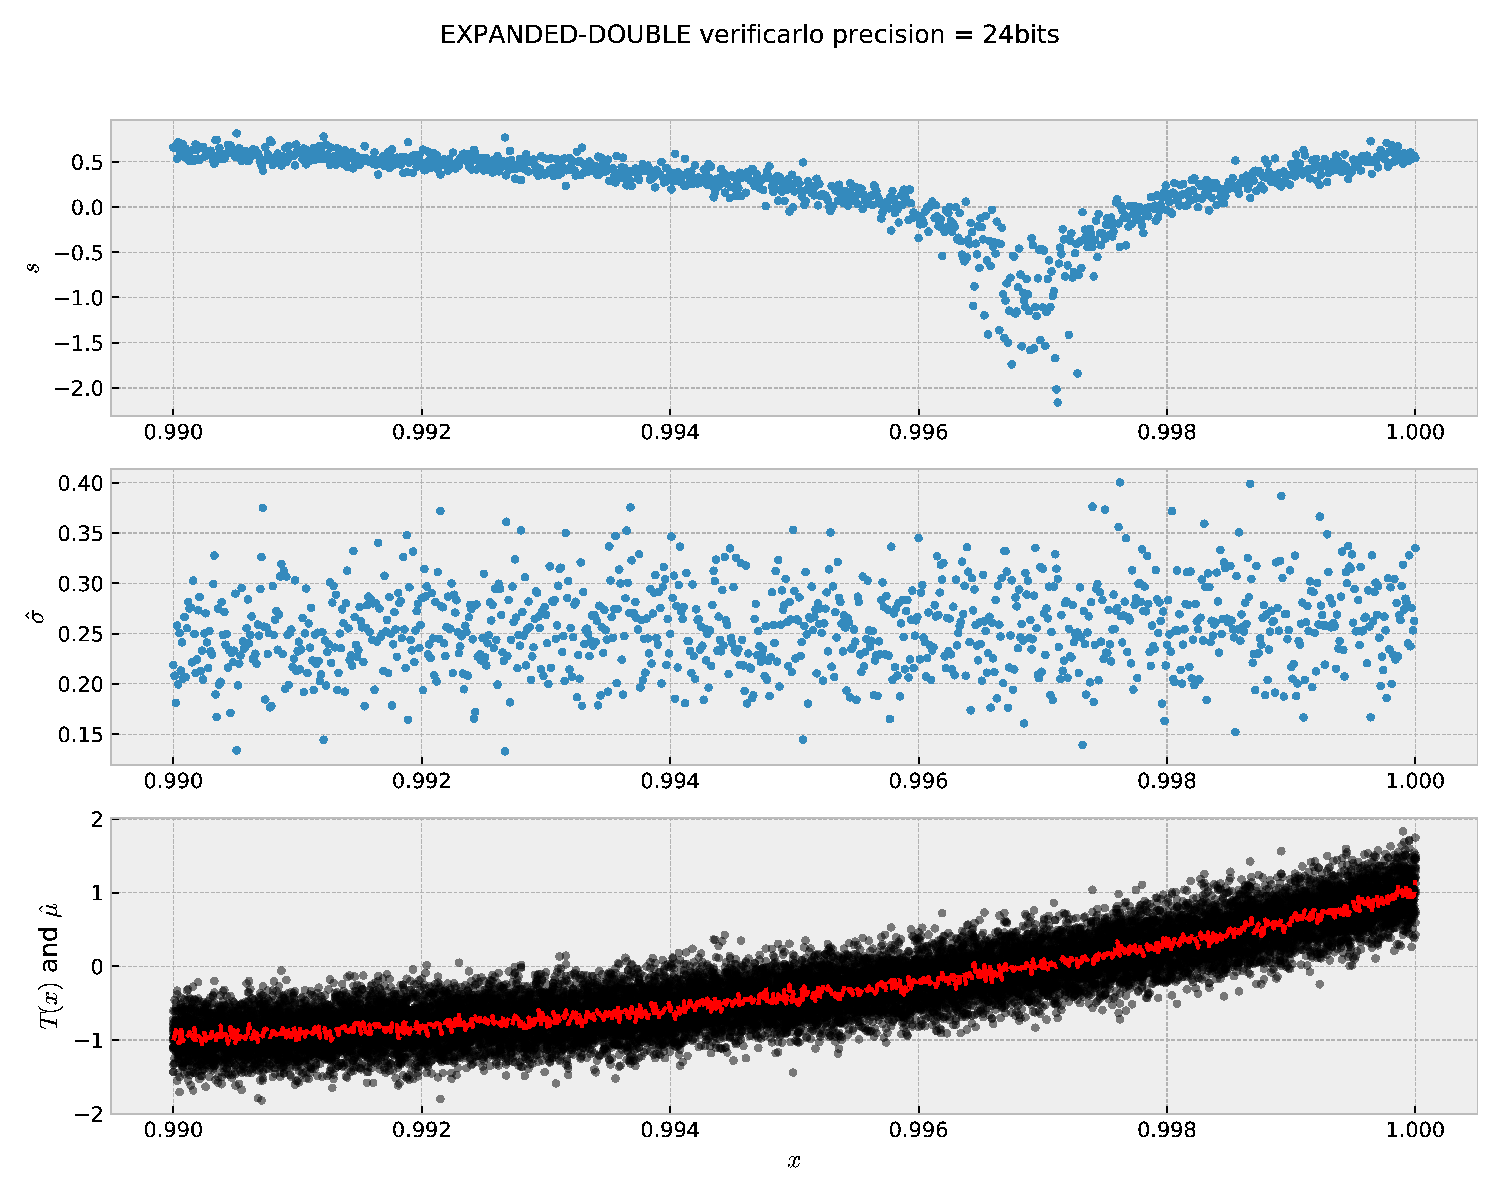
\includegraphics[width=.8\textwidth]{EXPANDED-DOUBLE-24-zoom.pdf}
  \caption{Evaluation of T(x) in its expanded form, compiled in double
    precision, with a virtual precision of 24}
  \label{fig:expanded:double:24:zoom}
\end{figure}

\begin{figure}[h]
  \center 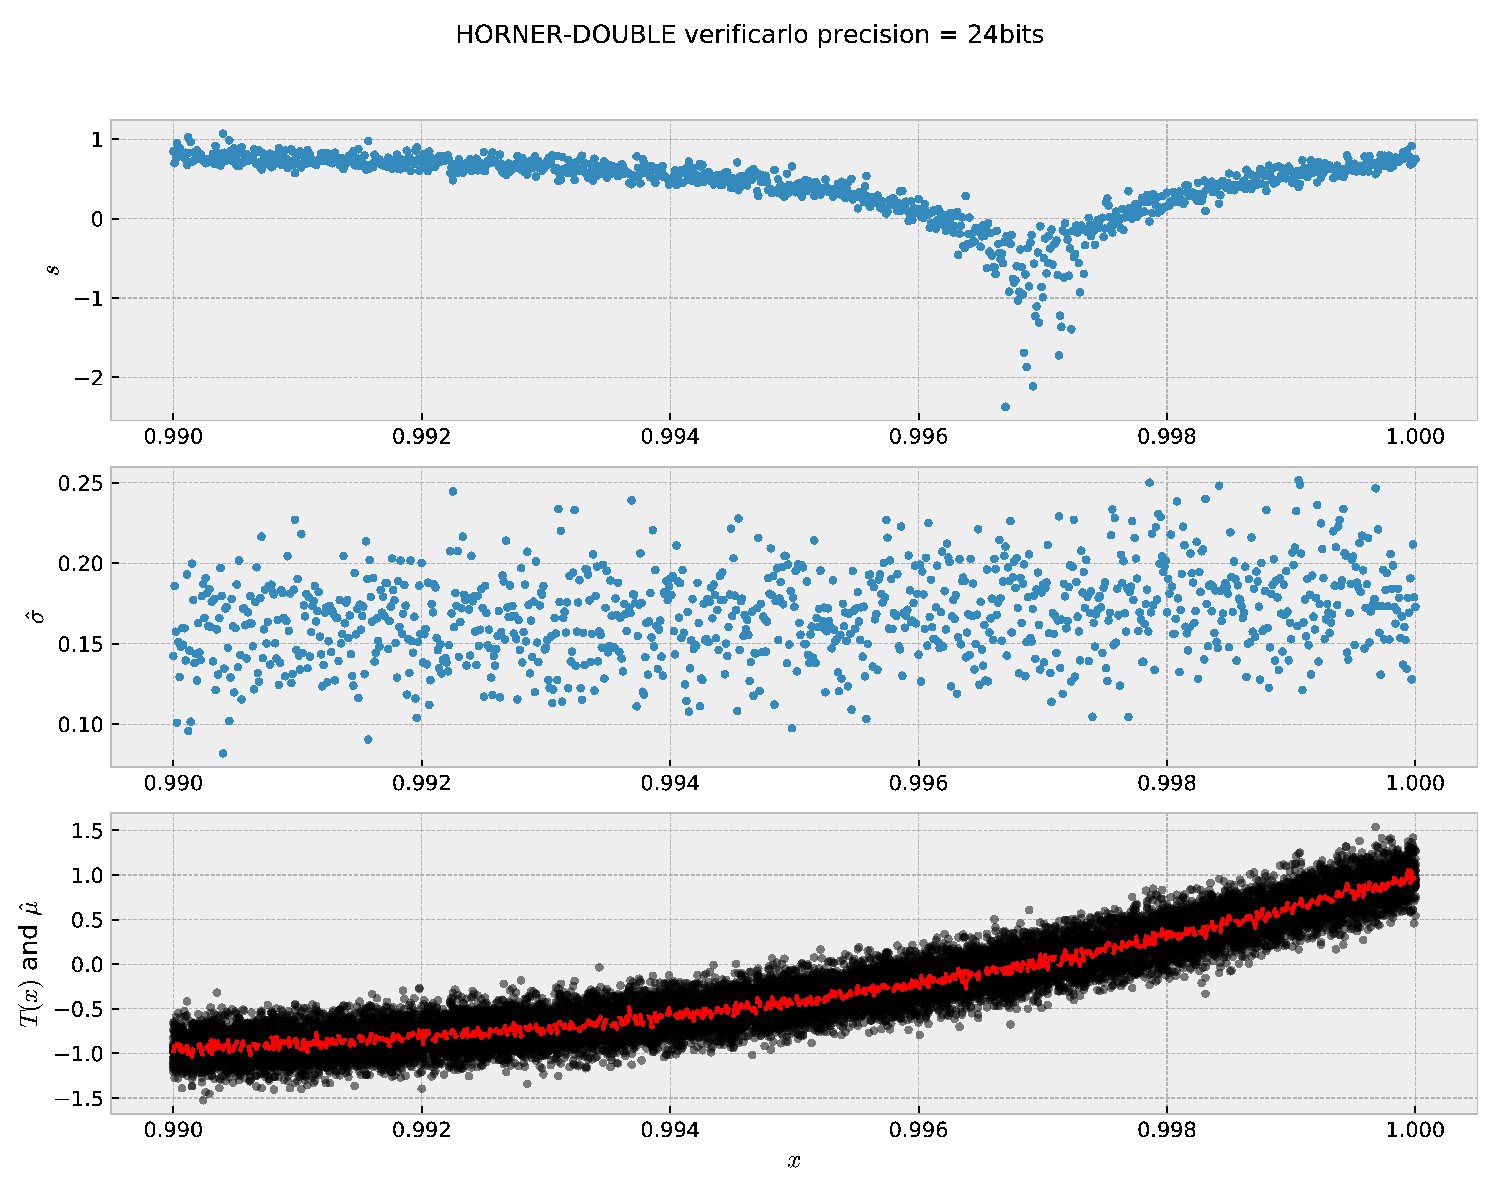
\includegraphics[width=.8\textwidth]{HORNER-DOUBLE-24-zoom.pdf}
  \caption{Evaluation of T(x) using Horner scheme, compiled in double precision,
    with a virtual precision of 24}
    \label{fig:horner:double:24:zoom}
\end{figure}


%% Uncomment below lines to include the extra Horn Compensated analysis
\FloatBarrier
\subsection{BONUS: Compensated Horner's method}
This section contains a Bonus exercice on the Compensated Horner's Method.
The goal is to demonstrate how Verificarlo can be used to compare different evaluation methods and how it interact with numerical functions available through library calls.
 

"Compensated" algorithms belongs to the class of algorithms that increase
program precision without changing the internal working format. 
The goal is to capture for each operation an estimation of the error term and to reinject it into the result.
For the Horner scheme, it is possible to retrieve at every step the error in
$x^2$ and the addition of the next coefficient by using respectively the
$Veltkamp-Dekker$ ({\tt twoProd}) for the product and $twoSum$ for the sum.
These algorithm are qualified as ({\it Error Free Transform}), EFT, in the
literature. 
The algorithm for the compensated horner scheme described in \cite{graillat2005compensated} is:

\begin{algorithmic}[1]
  \Procedure{compHorner}{$x$,$\{a_1, a_2, \ldots, a_n\}$}
    \State {$s_n \gets a_n$}
    \State {$r_n \gets 0$}
    \For {$i \in [n-1:0]$}
       \State $[p_i, pe_i] \gets \text{\sc TwoProd}(s_{i+1}, x^2)$
       \State $[s_i, se_i] \gets \text{\sc TwoSum}(p_i, a_i)$
       \State $r_i \gets r_{i+1}\times x^2+(pe_i+se_i)$
    \EndFor
    \State \Return $s_0 + r_0$
  \EndProcedure
\end{algorithmic}

The lines 5 and 6, evaluates HORNER with EFT calls. Line 7 accumulate the error terms, which will be added to the final result in line 9.

\begin{question}
  \begin{enumerate}[(a)]
    \item Modify {\tt run.sh} to call comphorner with the following command: {\tt ./run.sh COMPHORNER FLOAT 24 }.
  \end{enumerate}
\end{question}

Instead of (carefully) recoding EFTs {\sc TwoProd} and {\sc TwoSum} manually, we suggest to use {\tt libeft}~\cite{libeft} available and documented at the following address: \url{https://github.com/ffevotte/libeft}.

\begin{question}
  \begin{enumerate}[(a)]
    \item Modify {\tt run.sh} to add libeft to the linker command. For this, just add {\tt -left} to verificarlo command and ensure that libeft path is in your  {\tt LIBRARY\_PATH}.
    \item Modify {\tt tchebychev.c} following that example:

      {
      \begin{lstlisting}[style=customC, basicstyle=\normalsize]
      #include <libeft.h>

      /* Define real type and format string */
      #ifdef DOUBLE
      #define REAL double
      #define FMT "%.16e %.16e"
      #define TWOPROD twoprod_d
      #define TWOSUM  twosum_d
      #else
      #define REAL float
      #define FMT "%.7e %.7e"
      #define TWOPROD twoprod_s
      #define TWOSUM  twosum_s
      #endif
      \end{lstlisting}
      }

     These modifications allow defining two macros corresponding to  {\tt TWOPROD} and {\tt TWOSUM} calling the EFT version according to the floating point format you are using.


    \item Implement {\tt REAL compHorner(REAL x)} in {\tt tchebychev.c} according to the comphorner algorithm provided in this tutorial. Modify the {\tt main} function to allow calling comphorner.
    \end{enumerate}
\end{question}


\begin{question}
  Evaluate {\tt compHorner} precision with Verificarlo. What happens if you use a precision different from 53 for program compiled in DOUBLE precision?

  $\Rightarrow$ WARNING, {\sc TwoProd} and {\sc TwoSum} relies on exact operations; it is essential to use RR 53 (Random Rounding with precision 53) mode of verificarlo for  \texttt{double} or RR 24 for \texttt{float}.
  \\~\\
  You should get the results of figures~\ref{fig:comphornerVerificarlo24_53}.
\end{question}


\begin{table}
\begin{tabular}{cc}
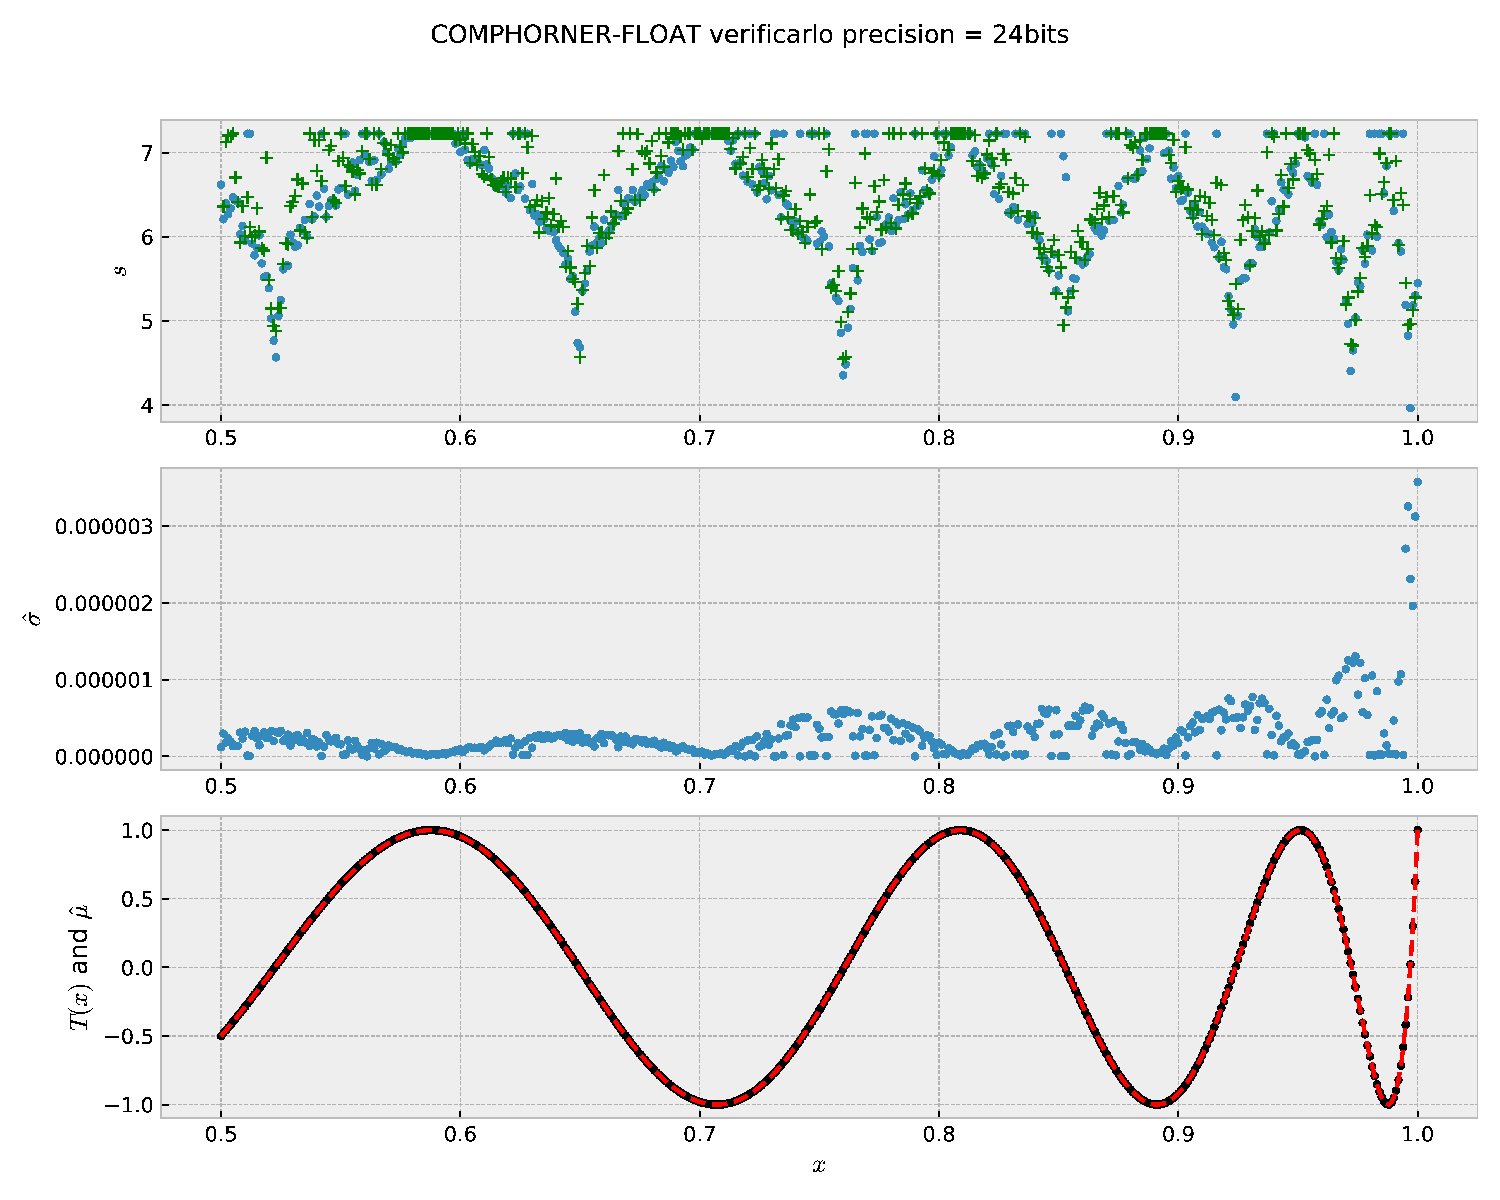
\includegraphics[width=.47\textwidth]{COMPHORNER-FLOAT-24+err.pdf}& 
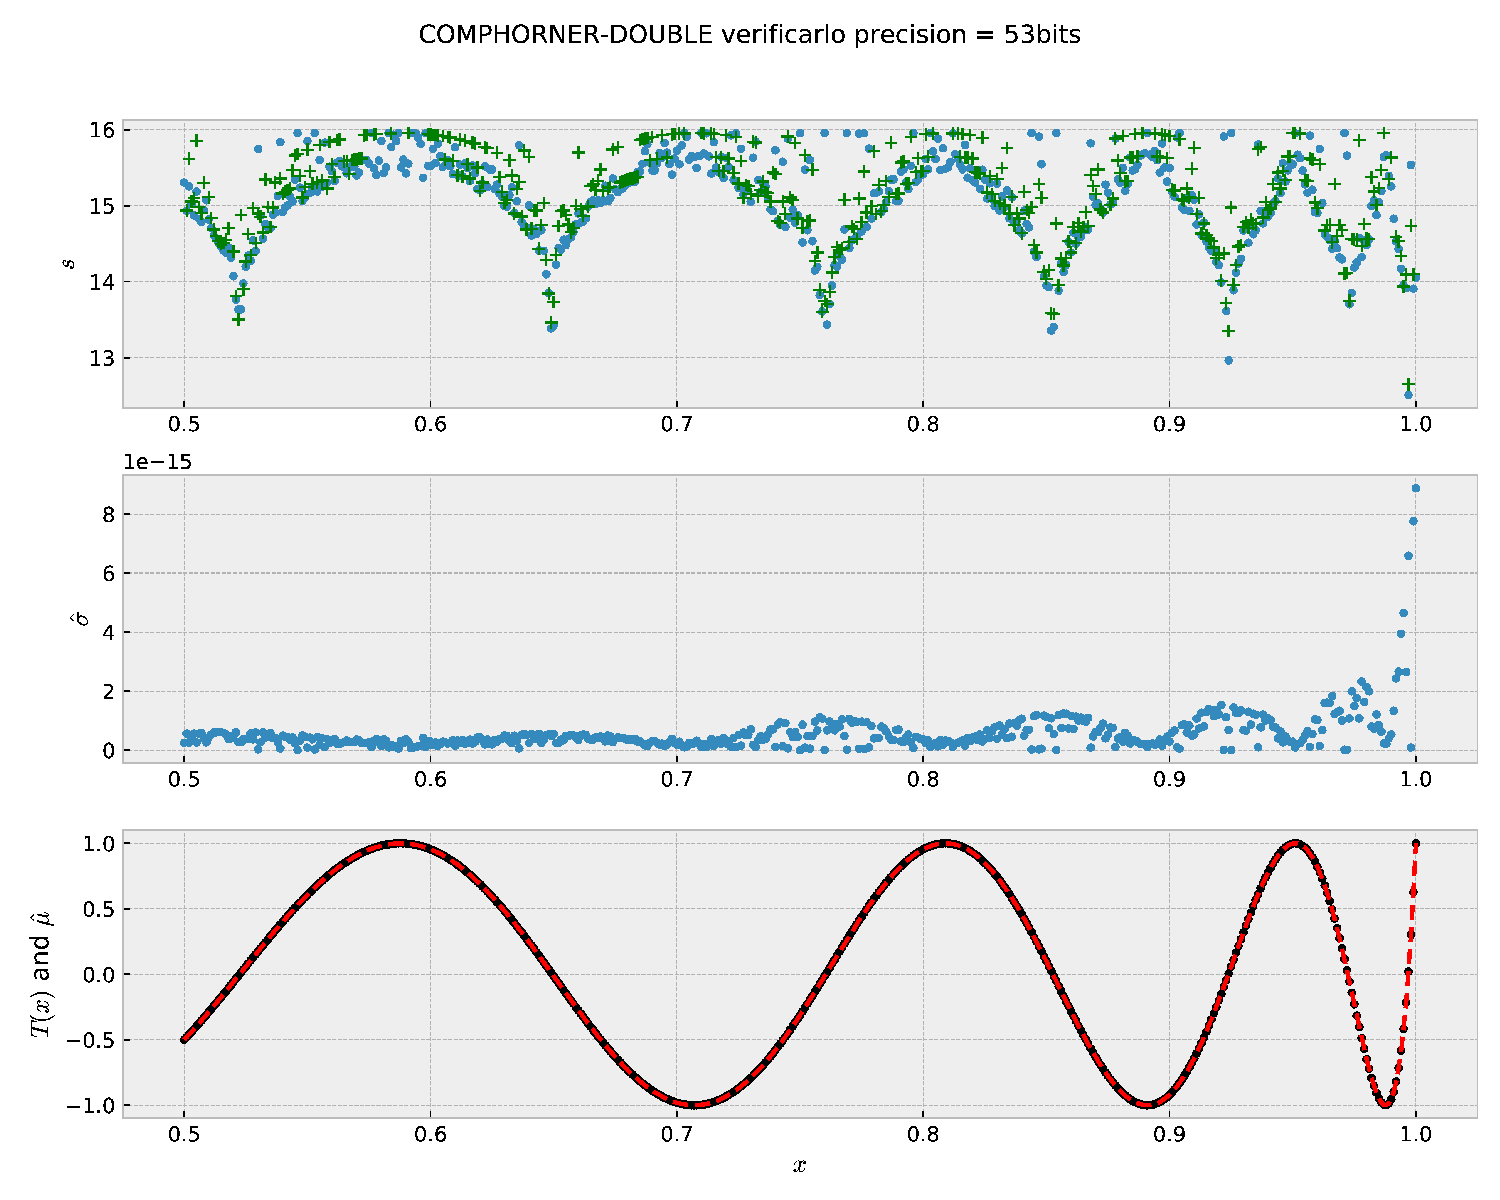
\includegraphics[width=.47\textwidth]{COMPHORNER-DOUBLE-53+err.pdf}\\
\end{tabular}
  \caption{Evaluation of T(x) using Horner and compHorner in single/double (left/right) precision: error estimated by verificarlo (blue), compared to the real error (green)}
  \label{fig:comphornerVerificarlo24_53}
\end{table}


The resulting precision of this approach are given in figures~\ref{fig:comphornerVerificarlo24_53} with verificarlo. 
Filled circles represent the real error value (evaluating in rational arithmetic in Python); circles represent the quality of the result computed in Monte Carlo Arithmetic with Verificarlo~\cite{verrou}.

We can notice on these figures that CompHorner compensate precision losses in double and single precision. We retrieve a behavior similar to the factored form, in particularly for points $T(x)=1$. However, knowing the polynomial's roots for using the Horner scheme is not required.

Out of these plots, we can make two interesting observations.
First, at the cost of an increasing number of operations, (but generally in the same complexity class) it is possible to recover a part (or the full) precision losses. There are algorithms called "accurate" that compute result without loss of precision, by, for example, recursively keeping errors terms until they can not be represented in the final result and such that rounding is correct ({\it e.g.} $accSum$ of S. Hump).

Second, some algorithms, especially in mathematical libraries (libmath, Intel MKL, Intel VML, libeft) used particularity of the floating-point format. By using Monte Carlo Arithmetic, it can be difficult even impossible to analyze them. In the random rounding specific case (as implemented by verificarlo RR mode with a precision length(mantissa)+1), a large amount of compensated algorithms can be analyzed (including compHorner as seen before). In addition, by their design, these algorithms have a proof of their level's precision correctness, which makes their evaluation by empirical methods useless.




%% Uncomment the following line to include Veritracer in the tutorial
%% \FloatBarrier
%% \section{Using Veritracer}

During the first public presentation, J.M. Muller asked us if our tool could handle the following case illustrated in his book:

 \begin{equation}
   u_{n} = 111 - \dfrac{1130}{u_{n-1}} + \dfrac{3000}{u_{n-1}u_{n-2}}
   \label{eq:muller_sequence_un}
 \end{equation}

The fixed points of this sequence are the roots of the polynomial:

\quad $u^3 - 111u^2 + 1130u - 3000 = (u-5)(u-6)(u-100)$

With the chosen initial values, $u_0=2$ and $u_1=-4$, the mathematical answer is 6.

\subsection{Running the code with Veritracer}

We will first reproduce the experiment of D. Stott Parker~\cite{parker1997monte}.

\begin{question}
    \begin{enumerate}[(a)]
\item Compile and test {\tt muller.c}
\item Modify {\tt Makefile} to compile with {\tt verificarlo}
\item Collect 32 results with virtual precision 53.
\item Compute the number of significant digits $s$.

$\Rightarrow$ As you can see the program is converging to the dominant root of the polynomial {\it i.e.} 100, with maximum precision! Therefore, by looking only to the final precision one could conclude that this is the correct answer\\~\\

\end{enumerate}
\end{question}

We will now do the experiment with veritracer to better understand this result.

\begin{question}
    \begin{enumerate}
        \item Type the command {\tt verificarlo -{}-help} to print how to call veritracer usage
        \item Type the command, and check the output and the {\tt .map} generated files \newline
        {\tt verificarlo -{}-verbose -{}-tracer muller.c -o muller -{}-function muller1 }
        \item Remove the current location map and launch veritracer in backtrace mode with the following command: {\tt verificarlo -{}-verbose -{}-tracer muller.c -o muller -{}-function muller1  -{}-tracer-backtrace}
        \item Run the program in the tracer environment with the following command: \newline
        {\tt veritracer launch -{}-force -{}-binary muller -{}-jobs 29}
        \item Check the content of the {\tt .vtrace} directory
        \item To launch the trace analysis run the command: {\tt veritracer analyze } and check the result in  the file {\tt .vtrace/veritracer.000bt}
        \item Plot the result with the provided {\it ad-hoc} script with the following command: \newline
        {\tt veritracer plot .vtrace/veritracer.000bt}
        \item It is possible to add invocation information with the following command: \newline
        {\tt veritracer plot .vtrace/veritracer.000bt -{}-invocation-mode}
        \item and basic statistics: {\tt veritracer plot .vtrace/veritracer.000bt -{}-invocation-mode -{}-mean -{}-std}
%rm locationInfo.map
%verificarlo -{}-verbose -{}-tracer muller.c -o muller -{}-function muller1  -O3
%locationInfo.map -> vide Why ?

%verificarlo -{}-verbose -{}-tracer muller.c -o muller -{}-function muller1  -O3
%verificarlo -{}-verbose -{}-tracer muller.c -o muller -{}-function muller1
%-{}-tracer-backtrace -O3 -{}-tracer-level temporary
%cat locationInfo.map


%veritracer launch -{}-force -{}-binary muller -j 29
%veritracer analyze
%empty traces ? Pourquoi


%verificarlo -{}-verbose -{}-tracer muller.c -o muller  -{}-tracer-backtrace
%-O3 -{}-tracer-level temporary
    \end{enumerate}
    $\Rightarrow$ NEW update: a pre-release GUI to plot and navigate in the trace is available on github for a more friendly user experience
\end{question}

$\Rightarrow$ Figure~\ref{fig:muller_sequence_un} has been automatically generated thanks to veritracer. It shows the evolution of the significant digits with the iteration. We can observe a gradual degradation of the precision until it reaches no significant digits. Then the precision is gradually improving to reach the maximum attainable in double precision format, {\it i.e.} 17. This plot allow us to conclude that the generated results, while being precise, as lost all its accuracy.

For the final experiment of this section we will use veritracer on the Tchebychev polynomial from this tutorial.

\begin{question}
  \begin{enumerate}[(a)]
      \item Experiment veritracer on the Tchebychev Polynomial evaluation between $0$ and $1$ by $0.001$.
      $\Rightarrow$ The result is presented in figure~\ref{fig:veritcheby}.

%rm locationInfo.map
%verificarlo -{}-tracer tchebychev.c -o tchebychev -O3  -{}-tracer-level
%temporary -{}-tracer-backtrace
%cat locationInfo.map

%veritracer launch -{}-force -{}-binary "./tchebychev FACTORED 100" -j 29 &&
%veritracer analyze

%veritracer plot .vtrace/veritracer.000bt -{}-invocation-mode -{}-mean -{}-std
%
%cat locationInfo.map |grep factored| grep ret
%veritracer plot .vtrace/veritracer.000bt -{}-invocation-mode -{}-mean -{}-std
%-v $$

%cat locationInfo.map |grep horner| grep ret
%veritracer launch -{}-force -{}-binary "./tchebychev  HORNER 100" -j 29 &&
%veritracer analyze
%veritracer plot .vtrace/veritracer.000bt -{}-invocation-mode -{}-mean -{}-std
%-v $$

  \end{enumerate}
\end{question}

 \begin{figure}[h!]
  \centering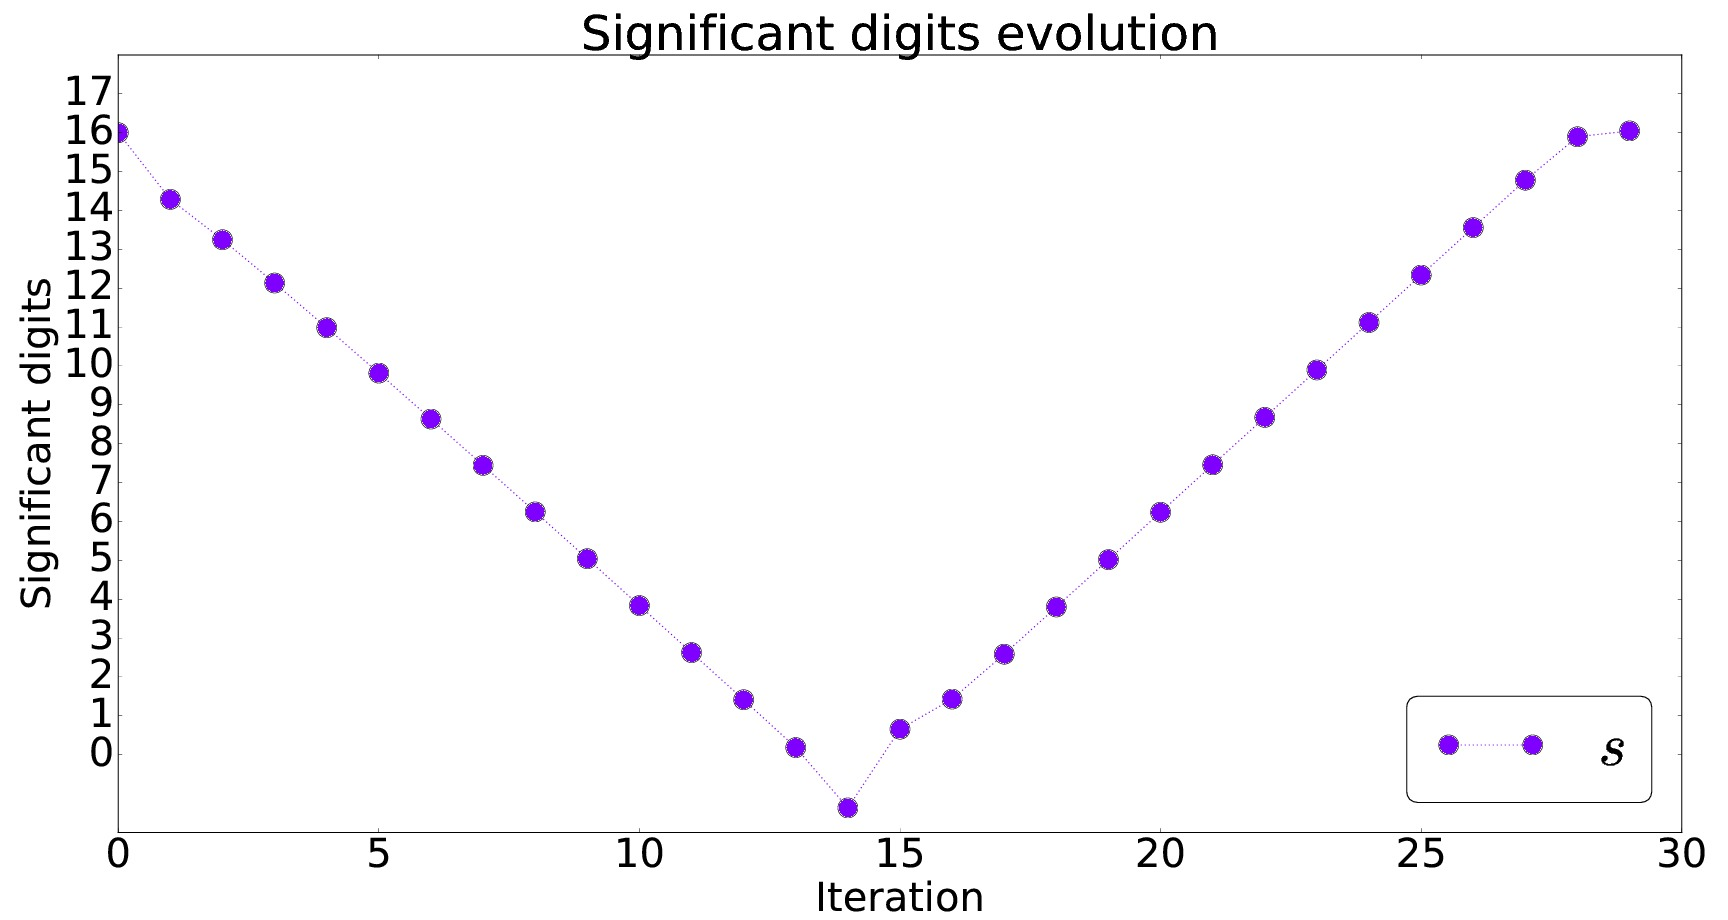
\includegraphics[width=0.8\linewidth]{muller_sequence_un.jpg}
  \caption{The evolution of the number of significant decimal digits ($s$) over time
     for the sequence $u_n$ in equation~\ref{eq:muller_sequence_un}.
    For $n=14$, $s$ is below 0 means that $u_{14}$ has no correct decimal digits.
     Only checking the final results is not enough to detect accuracy loss.
  }

 \label{fig:muller_sequence_un}
 \end{figure}
%
%
\begin{figure}[h!]
  \centering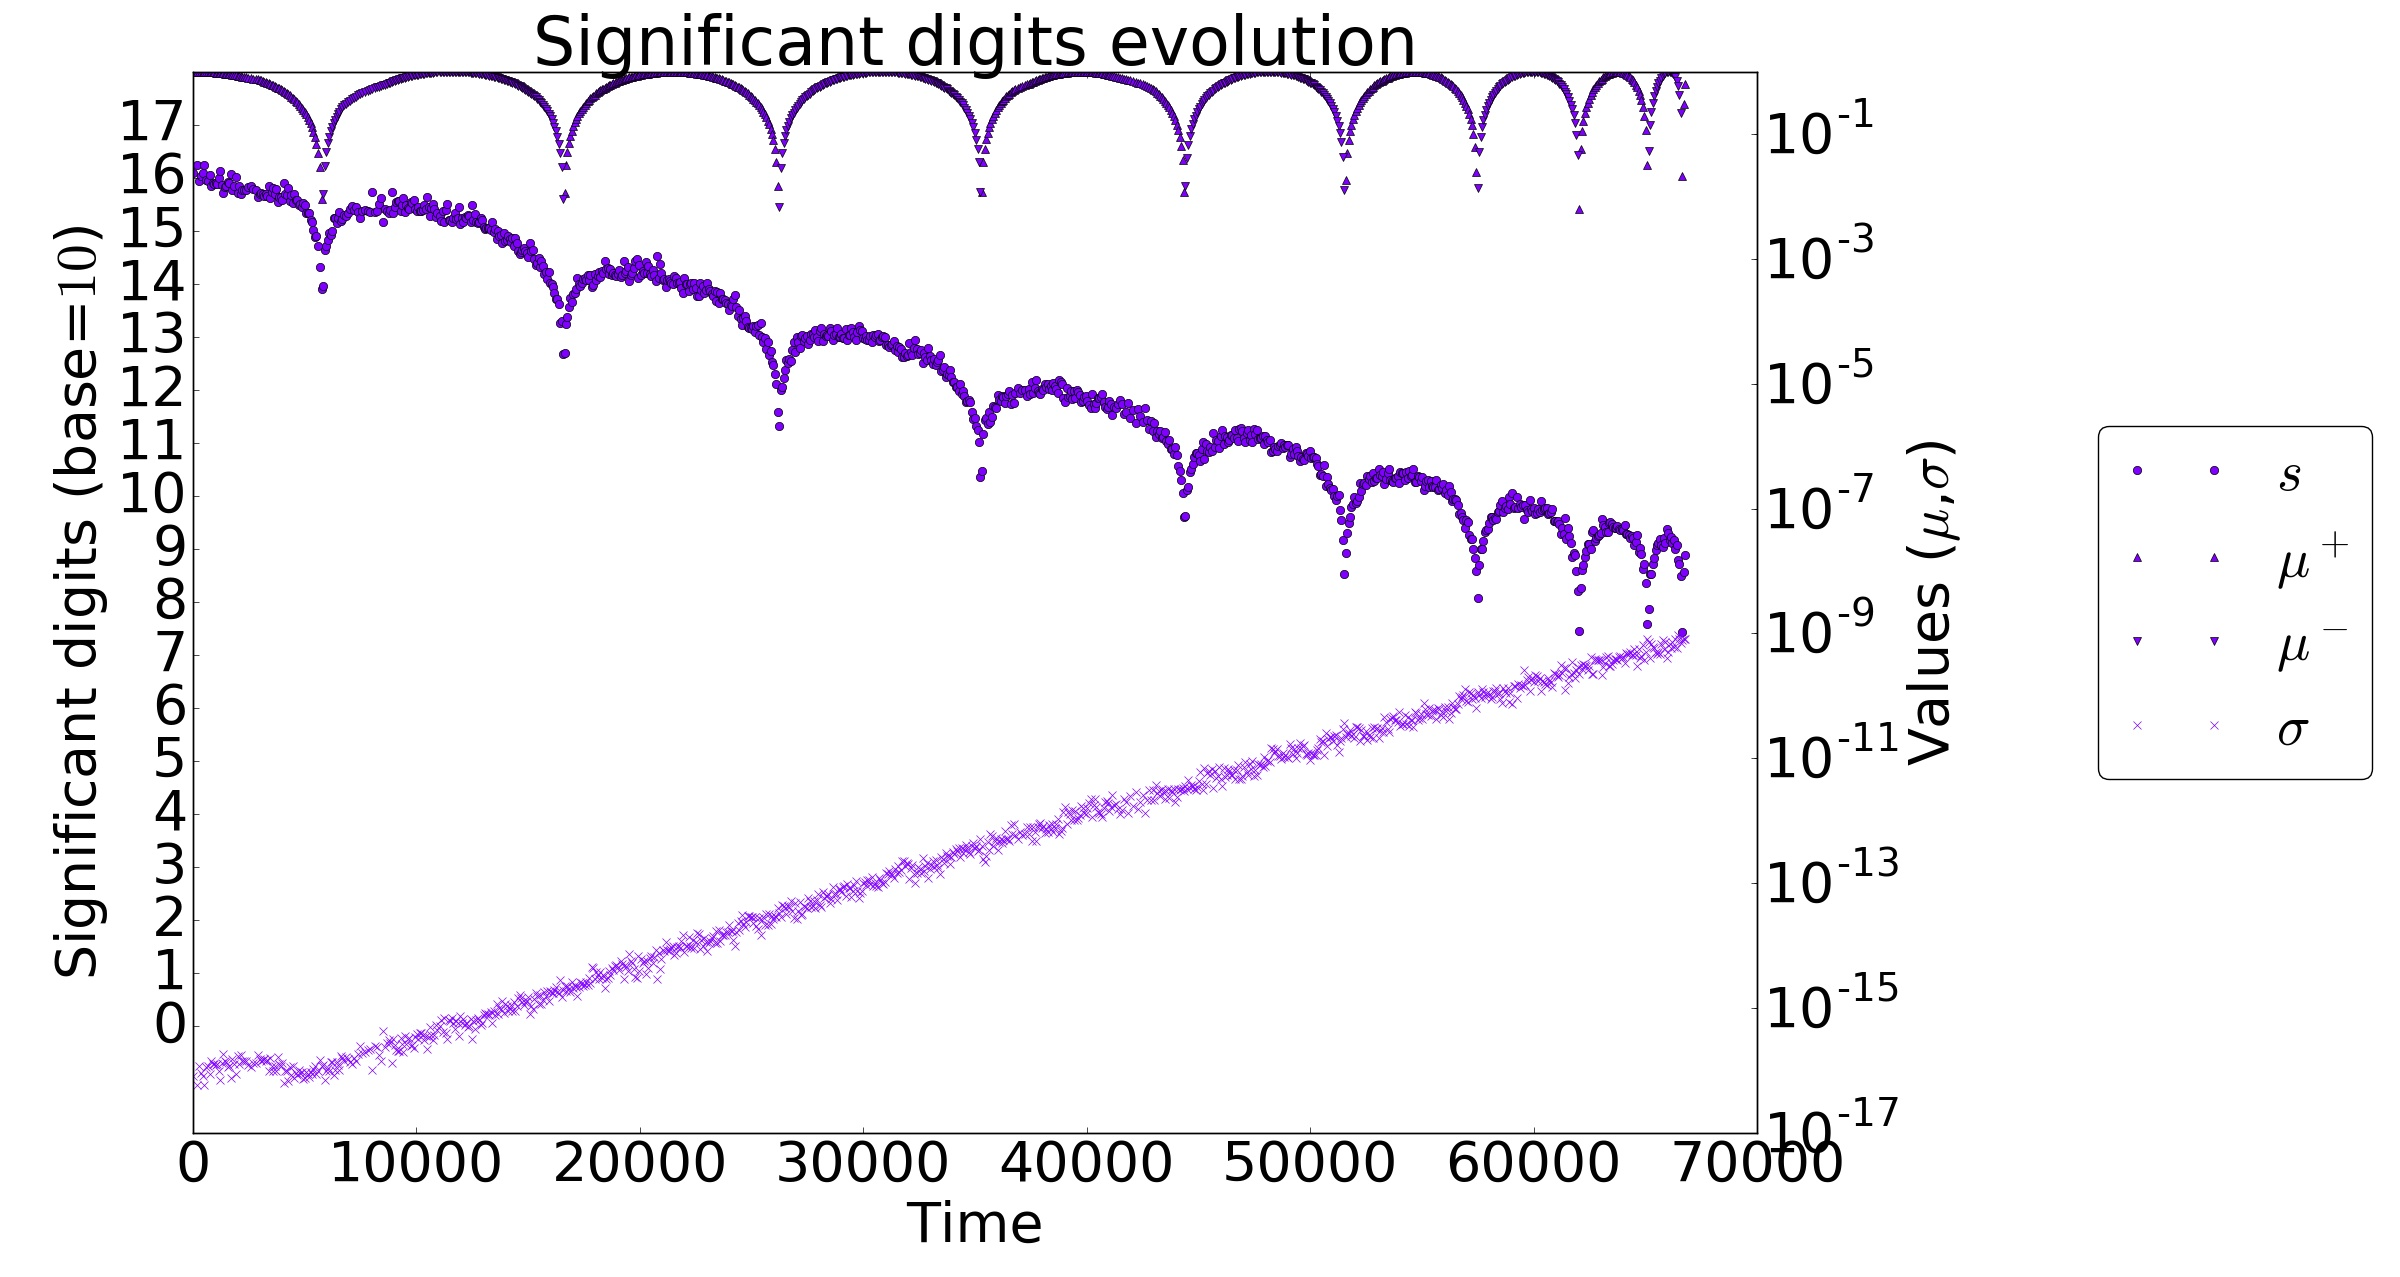
\includegraphics[width=1\linewidth]{tcheby_veritracer_large_font.jpg}
 \caption{The evolution of the number of significant decimal digits ($s$) over time
     for the evaluation of the tchebytchev polynomial used in this tutorial, from $0$ to $1$ by $0.001$.
  }
 \label{fig:veritcheby}
 \end{figure}
%
%
 ~\\~\\$\Rightarrow$ Veritracer contextualizes and traces variable precision over time: it helps to understand the arithmetic behavior of a program. It allows to focus program analysis on a limited set of functions, variables and inputs context.
%
%\FloatBarrier
%\clearpage



\FloatBarrier
\newpage
\bibliographystyle{ieeetr}
\bibliography{bibliography}

\end{document}
